\documentclass[a4paper] {report}
\usepackage{geometry}
\usepackage[utf8]{inputenc}
\usepackage[T1]{fontenc}
\usepackage[all]{xy}
\usepackage{textcomp, mathrsfs}
\usepackage{bm}
%\usepackage[french]{babel}
%\frenchbsetup{CompactItemize=false}
\usepackage{xcolor,epic,eepic,multicol, listings}
\usepackage{pstricks, pst-plot, enumitem}
\usepackage{amsmath,amssymb,amsfonts}
\usepackage[framed,thmmarks]{ntheorem}
\usepackage{ulem, eurosym}
\usepackage{graphicx, colortbl} 
\usepackage{bmpsize, comment}


\newcommand{\Z}{\mathbb{Z}}
\newcommand{\R}{\mathbb{R}}
\newcommand{\Q}{\mathbb{Q}}
\newcommand{\N}{\mathbb{N}}
\newcommand{\D}{\mathbb{D}}

\theorembodyfont{\upshape} 
\theoremheaderfont{\bfseries}
\theoremseparator{:} 

\newtheorem{defi}{\uline{D�finition}}[section]
\newcommand{\defin}[1]{\begin{defi}\begin{minipage}[t]{16.4}#1\end{minipage}\end{defi}\vspace{0.3cm}}
\newcommand{\defibox}[1]{\fbox{\begin{minipage}{\textwidth}\begin{defi}
\begin{minipage}[t]{16.4cm}#1\end{minipage}\end{defi}\end{minipage}}\vspace{0.3cm}}
\renewcommand{\thedefi}{\empty{}} 

\newtheorem{defis}{\uline{D�finitions}}[section]
\newcommand{\defins}[1]{\begin{defis}\begin{minipage}[t]{16.4}#1\end{minipage}\end{defis}\vspace{0.3cm}}
\newcommand{\defisbox}[1]{\fbox{\begin{minipage}{\textwidth}\begin{defis}
\begin{minipage}[t]{16.4cm}#1\end{minipage}\end{defis}\end{minipage}}\vspace{0.3cm}}
\renewcommand{\thedefis}{\empty{}} 

\newtheorem{theo}{\uline{Th�or�me}}[section]
\newcommand{\theor}[1]{\begin{theo}\begin{minipage}[t]{16.4cm}#1\end{minipage}\end{theo}\vspace{0.3cm}}
\newcommand{\theobox}[1]{\fbox{\begin{minipage}{\textwidth}\begin{theo}
\begin{minipage}[t]{16.4cm}#1\end{minipage}\end{theo}\end{minipage}}\vspace{0.3cm}}
\renewcommand{\thetheo}{\empty{}} 

%\newtheorem{propr}[theo]{\uline{Propri�t�}}
%\newcommand{\propri}[1]{\begin{propr}\begin{minipage}[t]{16.4cm}#1\end{minipage}\end{propr}\vspace{0.3cm}}
%\newcommand{\proprbox}[1]{\fbox{\begin{minipage}{\textwidth}\begin{propr}
%\begin{minipage}[t]{16.4cm}#1\end{minipage}\end{propr}\end{minipage}}\vspace{0.3cm}}
%\renewcommand{\thepropr}{\empty{}} 
%
%\newtheorem{proprs}[theo]{\uline{Propri�t�s}}
%\newcommand{\propris}[1]{\begin{proprs}\begin{minipage}[t]{16.4cm}#1\end{minipage}\end{proprs}\vspace{0.3cm}}
%\newcommand{\proprsbox}[1]{\fbox{\begin{minipage}{\textwidth}\begin{proprs}
%\begin{minipage}[t]{16.4cm}#1\end{minipage}\end{proprs}\end{minipage}}\vspace{0.3cm}}
%\renewcommand{\theproprs}{\empty{}} 

\newtheorem{propo}[theo]{\uline{Proposition}}
\newcommand{\propos}[1]{\begin{propo}\begin{minipage}[t]{16.4cm}#1\end{minipage}\end{propo}\vspace{0.3cm}}
\newcommand{\propobox}[1]{\fbox{\begin{minipage}{\textwidth}\begin{propo}
\begin{minipage}[t]{16.4cm}#1\end{minipage}\end{propo}\end{minipage}}\vspace{0.3cm}}
\renewcommand{\thepropo}{\empty{}} 

\newcommand{\thbox}[2]{\fbox{\begin{minipage}{\textwidth}\textbf{\uline{#1} : }
\begin{minipage}[t]{16.4cm}\upshape{#2}\end{minipage}\end{minipage}}\vspace{0.3cm}}

\newcommand{\sg}[1]{\textbf{\underline{#1}}}
\newcommand{\tsg}[1]{\textbf{\underline{#1} : }}

\renewcommand{\labelenumi}{\textbf{\arabic{enumi})}}
\renewcommand{\labelenumii}{\textbf{\alph{enumii})}}

\newcommand{\rem}[1]{\begin{flushleft}\textbf{\underline{Remarque} : }\begin{minipage}[t]{16.4cm} #1 \end{minipage}\end{flushleft}}
\newcommand{\rems}[1]{\begin{flushleft}\textbf{\underline{Remarques} : }\begin{minipage}[t]{16.4cm} #1 \end{minipage}\end{flushleft}}
\newcommand{\ex}[1]{\begin{flushleft} \textbf{\underline{Exemple} : }\begin{minipage}[t]{16.4cm} #1 \end{minipage} \end{flushleft}}
\newcommand{\exo}[3]{\begin{flushleft}{\bf\LARGE \underline{Exercice #1} : }{\footnotesize #2} {\bf \begin{minipage}[t]{14cm} #3 \end{minipage}} \vspace{0.3cm} 
\\\end{flushleft}}
\newcommand{\titre}[1]{\begin{center} \bf{\huge #1 }\end{center}\vspace{0.5cm}}

\setlength{\unitlength}{1cm}
\psset{arrowinset=0}

\definecolor{string}{rgb}{0.317,0.49,0.345}
%\definecolor{keyword}{rgb}{0.80,0.47,0.2}
%\definecolor{comments1}{rgb}{0,0.6,0}
\definecolor{comments2}{rgb}{0.37,0.55,0.32}
%\definecolor{fonctions}{rgb}{0,0.6,0}
\definecolor{attributs}{rgb}{0.59,0.43,0.56}
\lstset{		language=Python,
 				backgroundcolor=\color{white},
                basicstyle=\color{black}\small,
                keywordstyle=\color{orange}\ttfamily,
                stringstyle=\color{olive}\ttfamily,
                commentstyle=\color{gray}\ttfamily,
                morecomment=[s][\color{lime}]{/**}{**/},
                keepspaces=true,
                morekeywords={module, export, constructor, let, of, number}, 
                showstringspaces=false, 
                tabsize = 2,
                morekeywords={[2]taille, choix, nbIterations, geo, position, links, to, hashNumber, x, y, z}, 
                keywordstyle={[2]\color{attributs}},
                morekeywords={[3]go, goForTheFirstTime, getValue, allKeys, putValue, tan, angleBetweenTwoVectorsBetween0andPi, newFrom, substract, min, max, add, scale, push, setPosition },
                keywordstyle={[3]\color{yellow}}, 
                morekeywords={[4]0, 1, 2, 3, 4, 5, 6, 7, 8, "9"}, 
                keywordstyle={[4]\color{blue}}
}
\newrgbcolor{xdxdff}{0.49019607843137253 0.49019607843137253 1.}
\newrgbcolor{wwzzff}{0.4 0.6 1.}
\newcommand{\e}[1]{\bm{e_{#1}}}
\newcommand{\ei}{\e{\infty}}
\newcommand{\ez}{\e{0}}
\newcommand{\eu}{\e{1}}
\newcommand{\ed}{\e{2}}
\newcommand{\et}{\e{3}}

\renewcommand{\baselinestretch}{1.5}
\begin{document}

\psset{xunit=1cm, yunit=1cm, linewidth=1.1pt, plotpoints=300}
\renewcommand{\labelitemi}{$\bullet$}
\renewcommand{\labelitemii}{$-$}
\setlength{\leftmargini}{0.5cm}
\everymath{\displaystyle}
\graphicspath{{Images/}}
\let\oldref\ref
\renewcommand{\ref}[1]{(\oldref{#1})}
\renewcommand{\thesection}{\Roman{section})}
\renewcommand{\thesubsection}{\Roman{section}.\arabic{subsection})}
\renewcommand{\contentsname}{Sommaire}
\renewcommand{\bibname}{Bibliographie}
\title{Stage de M2 \\ - \\ Algèbres géométriques appliquées à la robotique en Coq\\ - \\ sous la direction de Julien Narboux }
\author{Jonathan Graff}
\date{Février - Juillet 2021}
\maketitle
\tableofcontents
\newpage

\section*{Remerciements}

Je tiens tout particulièrement à remercier mon tuteur de stage, Julien Narboux, pour sa sympathie et pour avoir pris le temps de m'expliquer tout ce domaine que je découvrais. Ses explications ont toujours été très claires, et je ne compte plus le temps passé ensemble à débugger les preuves en Coq.

Je remercie également Laurent Théry pour sa disponibilité et ses explications quant à sa bibliothèque que nous avons réutilisée, ainsi que pour le temps qu'il a passé à l'adapter à notre problème. 

Je remercie aussi Olivier Piccin pour ses explications sur les algèbres géométriques et sur la robotique en général. En particulier, son modèle réduit de robot 6R m'aura bien été utile. 

Enfin, je remercie en particulier ma femme pour son soutien indéfectible pendant toute cette année.

\addcontentsline{toc}{section}{\protect\numberline{}Remerciements}
\newpage
\section{Introduction}
\subsection{Présentation de la structure}

Mon stage s'est déroulé au laboratoire ICube, situé à Illkirch. Ce laboratoire de recherche a été créé en 2013 par l'Université de Strasbourg, le SNRS, l'INSA et l'ENGEES.
Ce laboratoire regroupe des chercheurs dans "le domaine des sciences de l'ingénieur et de l'informatique avec l'imagerie comme thème fédérateur. Les champs d'application privilégiés sont l'ingénierie pour la santé, l'environnement et le développement durable."\cite{icube}

Ce laboratoire regroupe plus de 650 membres. Il est divisé en quatre équipes de recherche : 

\begin{itemize} 
\item le Département Imagerie, Robotique, Télédétection et Santé (D-IRTS)
\item le Département Électronique du Solide, Systèmes et Photonique (D-ESSP)
\item le Département Mécanique (D-M)
\item le département Informatique Recherche (D-IR), au sein duquel j'ai effectué mon stage. 
\end{itemize}
Il y a au total 14 équipes de recherche réparties dans ces quatre départements. J'ai effectué mon stage dans l'équipe "Informatique Géométrique et Graphique" (IGG). 

\subsection{Contexte}
\subsubsection{Algèbres géométriques}

Les algèbres géométriques sont un formalisme mathématique permettant de décrire de façon plus uniforme la géométrie 3D. Dans cet espace, les points, les vecteurs, les plans, les sphères, les cercles, les droites, ainsi que d'autres objets géométriques, mais aussi les transformations usuelles, sont tous représentés par le même objet : \textbf{un multivecteur}.
Cela simplifie grandement les notations puisque tous les calculs pourront se faire dans cette algèbre. Un autre avantage est que les cas particuliers sont inexistants, par exemple le calcul permettant d'obtenir un plan à partir de deux vecteurs renverra $0$ si les deux vecteurs sont colinéaires, il n'y a donc pas besoin de vérifier avant de construire notre plan que les vecteurs sont bien dans la configuration souhaitée. Egalement, ces algèbres incluent les nombres complexes de manière naturelle, mais aussi l'ensemble des quaternions. 

Tous ces avantages font qu'en pratique ces algèbres sont très utilisées dans plusieurs domaines : surtout en physique (mécanique classique et quantique, théories électromagnétiques et de la relativité...), mais aussi en biomécanique, pour la dynamique des vols spatiaux, la vision par ordinateur, et dans le domaine qui va nous intéresser ici : la robotique et plus précisément la robotique médicale.

\subsubsection{Assistant de preuve}

Les algorithmes implémentés dans des machines peuvent être vérifiés ou non. Par exemple, dans une voiture, ils ne le sont pas. Il n'est pas rare donc de trouver plusieurs centaines de millions de lignes de code pour un logiciel embarqué. Par contre, pas question de fonctionner ainsi dans un avion par exemple. Ici, chaque ligne de code doit être prouvée, il faut démontrer qu'aucun bug ne peut apparaître et faire crasher l'avion. Pour ce faire, on utilise un logiciel d'assistant de preuve qui va vérifier chaque ligne. Prouver un algorithme est en général bien plus long et fastidieux que de le créer, et donc par conséquent le nombre de lignes de code est beaucoup plus restreint, de l'ordre de cent mille pour un avion ou une fusée \cite{nblignescode}.  
Mais cela a une utilité réelle. Par exemple, le 4 juin 1996, le vol 501 de la fusée Ariane s'est écrasé seulement 36.7 secondes après son décollage. Le problème est venu d'un bug informatique de dépassement d'entier dans les registres mémoire des calculateurs électroniques utilisés par le pilote automatique. La fusée transportait quatre satellites d'une valeur de 370 millions de dollars, heureusement aucun humain n'a péri \cite{ariane}. Mais cela a montré l'importance de la preuve en informatique dans certains domaines. Si les codes avaient été prouvés à l'aide d'un logiciel assistant de preuve à ce moment-là, l'incident aurait très probablement été évité. 

\subsection{Objectifs}

En robotique médicale, aujourd'hui, il n'existe pas d'obligation de prouver les algorithmes régissant la mécanique des robots. Pourtant ceux-ci peuvent exécuter des opérations très complexes, et il serait donc souhaitable que ces algorithmes soient prouvés afin d'être sûr que le robot ne va pas faire quelque chose de non désiré. On peut aisément imaginer les catastrophes que cela engendrerait.  

L'objectif de mon stage est donc dans un premier temps de me familiariser avec le logiciel Coq, afin de comprendre comment celui-ci fonctionne puis dans un second temps, de me familiariser avec le concept des algèbres géométriques, concept complètement nouveau pour moi. Enfin, l'objectif est de réutiliser les bibliothèques d'algèbres géométriques de Laurent Théry, afin de les spécialiser pour faire de l'algèbre géométrique conforme, de prouver quelques théorèmes simples, et de prouver en utilisant certains robots connus que le bras de robot se trouve bien à la fin là où il est souhaitable qu'il aille, et pas ailleurs !

\section{Les algèbres géométriques}

\subsection{Présentation générale}

\subsubsection{Définitions}

L'algèbre géométrique $\mathscr{G}^n$ peut être vue comme une extension de l'espace vectoriel $\R^n$. Les objets de cet algèbre sont appelés \sg{multivecteurs}. L'algèbre possède donc une somme, prolongeant la somme classique des vecteurs, mais elle possède également un produit, appelé \sg{produit géométrique} et vérifiant les axiomes d'une algèbre unitaire associative. Le produit de deux multivecteurs $a$ et $b$ se note $ab$. Ce produit possède un élément neutre, noté $\bm{1}$ et possède la propriété que tout carré est un nombre réel.  

On peut déjà remarquer qu'on a alors : \begin{itemize}
\item $\R^n \subset \mathscr{G}^n$
\item $\R \subset \mathscr{G}^n$
\end{itemize}

On définit le \sg{produit scalaire} (ou produit intérieur) par la formule : $$\boxed{a \cdot b =  \frac{1}{2} (ab+ba)}$$

Ce produit scalaire définit une norme avec $||a||^2 = a \cdot a$.

On dira que deux multivecteurs sont \sg{orthogonaux} si leur produit scalaire est nul. 

On définit également le \sg{produit extérieur} par la formule $$\boxed{a \wedge b = \frac{1}{2} (ab-ba)}$$

Ainsi, le produit extérieur est anti-commutatif : $a \wedge b  = -b \wedge a $.

Avec ces formules, on remarque qu'on a : \\
\begin{equation*}
\boxed{\begin{array}{ll}
\textbf{Formule fondamentale : }&ab = a \cdot b + a \wedge b \\
\textbf{Anticommutativité : } &\text{Si }a \text{ et } b \text{ sont orthogonaux, alors }ab = -ba.
\end{array}}
%\label{fondamental}\label{anticomm}
\end{equation*} 

Dans toute la suite, nous noterons en gras et en lettre minuscule les vecteurs. 

Si $\lbrace \bm{e_1},\cdots, \bm{e_n} \rbrace$ est une base orthonormée de $\R^n$, on a les propriétés suivantes : 

$\bullet$ $\wedge$ est linéaire et associatif.

\begin{flalign}
&\hspace*{0.43cm}  \bullet \bm{e_i} \wedge \bm{e_j} = \left \lbrace \begin{array}{rl}
0 &\text{ si } i=j\\
\bm{e_i}\bm{e_j} & \text{ si } i\neq j
\end{array} \right.\label{wedgeprop} & &
\end{flalign}


\begin{flalign}
&\hspace*{0.43cm}  \bullet  \bm{e_i}\bm{e_j} =  \left \lbrace \begin{array}{rl}
1 &\text{ si } i=j\\
\bm{e_i} \wedge \bm{e_j} & \text{ si } i\neq j
\end{array} \right.\label{prodprop} & &
\end{flalign}

Les nouveaux éléments construits  $\bm{e_i} \bm{e_j}$ appartiennent donc à $\mathscr{G}^n$, mais ne sont pas des vecteurs de $\R^n$.

On peut également voir que $\mathscr{G}^n$ est un espace de dimension $2^n$, une base étant formée par $1$ et l'ensemble des produits de vecteurs distincts : $\lbrace 1, \bm{e_1}, \cdots, \bm{e_n}, \bm{e_1} \bm{e_2}, \bm{e_1}  \bm{e_3}, \cdots \bm{e_{n-1}} \bm{e_n}, \bm{e_1} \bm{e_2}  \bm{e_3}, \cdots, \bm{e_1}\cdots \bm{e_n}\rbrace$.

Pour simplifier les notations, l'élément $\bm{\bm{e_i}} \wedge \bm{\bm{e_j}} = \bm{\bm{e_i}\bm{e_j}}$ sera noté par la suite $e_{ij}$.

\subsubsection{Bivecteurs - Interprétation géométrique}

Prenons deux vecteurs $\bm{a}$ et $\bm{b}$. Si les deux vecteurs sont colinéaires, alors le produit extérieur de ces deux vecteurs sera nul. En effet, si $\bm{a} = \sum_{i=1}^n \lambda_i \bm{e_i}$ et $\bm{b}=C\sum_{j=1}^n \lambda_j \bm{e_j}$, alors : \\
 $\bm{a} \wedge \bm{b} = 
 C \left(\left(\sum_{i=1}^n \lambda_i \bm{e_i} \right)  \wedge  \left(\sum_{j=1}^n \lambda_j \bm{e_j}\right)\right) 
 = C \left( \sum_{i=1}^n \sum_{j=1}^n \lambda_i\lambda_j (\bm{e_i} \wedge \bm{e_j})\right) $ par linéarité
 
$= C\sum_{i=1}^n \sum_{j=1}^{i-1} \lambda_i\lambda_j (\bm{e_i} \bm{e_j} + \bm{e_j} \bm{e_i})$ d'après \ref{wedgeprop}

$= 0 $ par anti-commutativité.

Les éléments de l'algèbre géométrique $\mathscr{G}^n$ formés par le produit extérieur entre deux vecteurs non colinéaires sont appelés des \sg{bivecteurs}. C'est un cas particulier de multivecteurs. 

Géométriquement, dans un espace vectoriel euclidien, un vecteur définit une droite et sa norme est la longueur d'un segment de cette droite. Pour un bivecteur, c'est similaire :  on peut imaginer un bivecteur $\bm{u} \wedge \bm{v}$ comme définissant le plan vectoriel engendré par $\bm{u}$ et $\bm{v}$, et sa norme est une partie de l'aire de ce plan : c'est exactement l'aire du parallélogramme engendré par $\bm{u}$ et $\bm{v}$. Un bivecteur possède également une orientation : celle de $\bm{u}$ vers $\bm{v}$.

\begin{figure}[!ht]
\centering
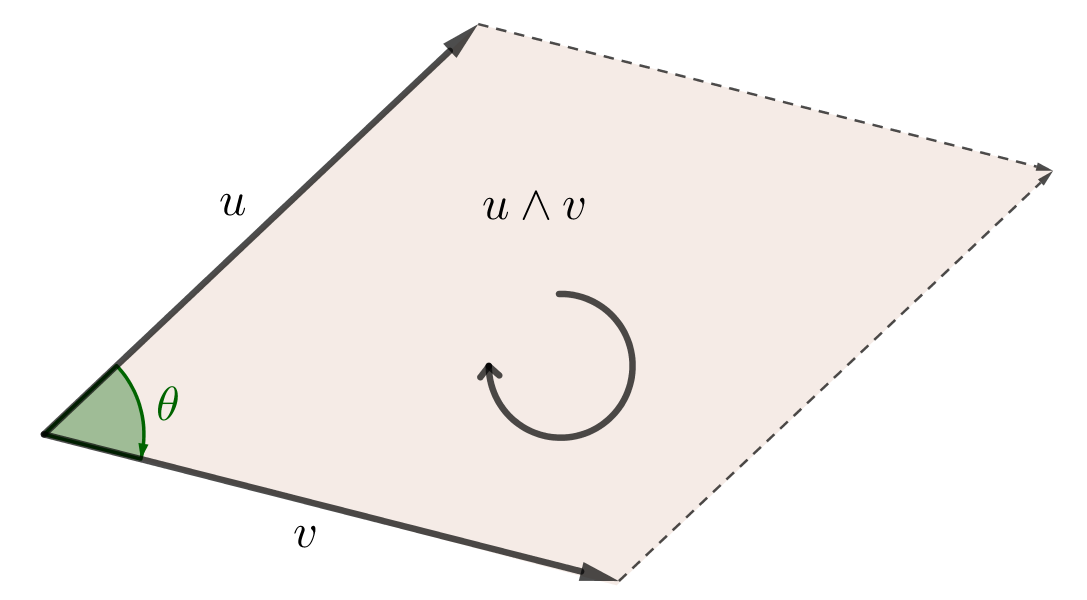
\includegraphics[scale=0.3]{bivecteur.png}
\caption{Un bivecteur}
\label{bivecteur}
\end{figure}

Au passage, on peut aussi noter la formule du parallélogramme $$||\bm{u} \wedge \bm{v}|| = ||\bm{u}||\cdot||\bm{v}||\cdot \sin (\bm{u};\bm{v})$$

\subsubsection{Egalité de bivecteurs}

Deux vecteurs sont égaux s'ils ont même direction, même sens et même norme, pour des bivecteurs c'est pareil : deux bivecteurs $\bm{a}\wedge\bm{b}$ et $\bm{c}\wedge\bm{d}$ sont égaux si et seulement si ils définissent le même plan, ont la même orientation et ont la même norme. Au final, pour les représenter géométriquement, on doit tracer une partie du plan formé par les deux vecteurs, de même aire que leur parallélogramme et de même orientation. Ainsi, ces bivecteurs-là sont par exemple égaux : 

\begin{figure}[!ht]
\centering
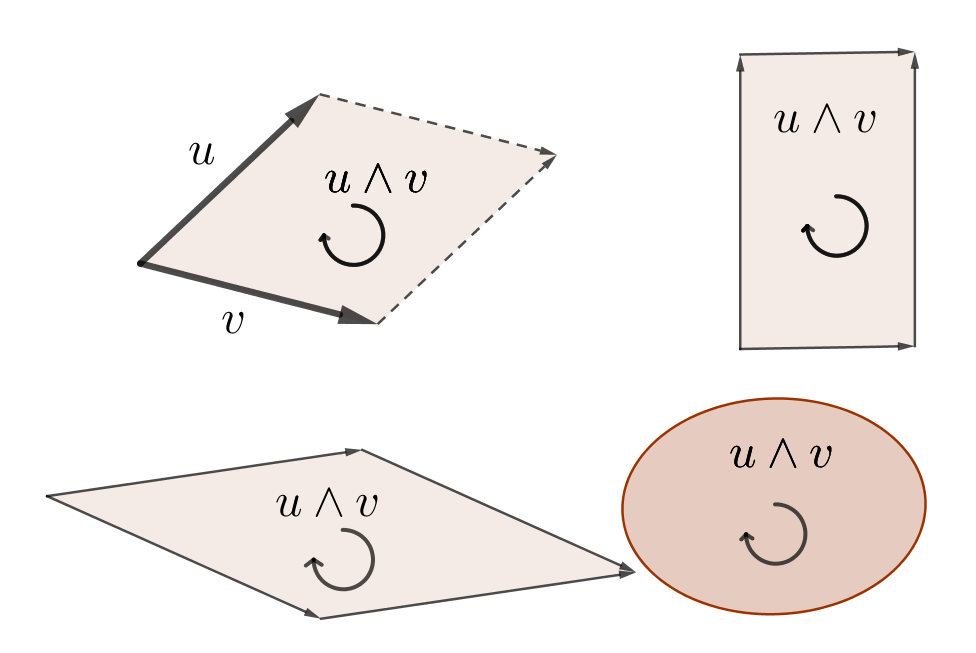
\includegraphics[scale=0.3]{egalite.png}
\caption{Egalité de bivecteurs}
\label{egalite}
\end{figure}

\subsubsection{Somme de bivecteurs}

Pour additionner deux bivecteurs $M_1 = \bm{a}\wedge\bm{b}$ et $M_2 = \bm{c}\wedge\bm{d}$ dont les plans induits ont une intersection, on procède comme suit :
\begin{itemize}
\item on modifie si nécessaire un ou deux bivecteurs de façon à ce que deux vecteurs soient identiques (c'est toujours possible si les plans s'intersectent), on a donc deux bivecteurs $\bm{u}\wedge\bm{w}$ et $\bm{w}\wedge\bm{v}$
\item Le résultat sera le bivecteur $(\bm{u}+\bm{v})\wedge\bm{w}$
\end{itemize}

\begin{figure}[!ht]
\centering
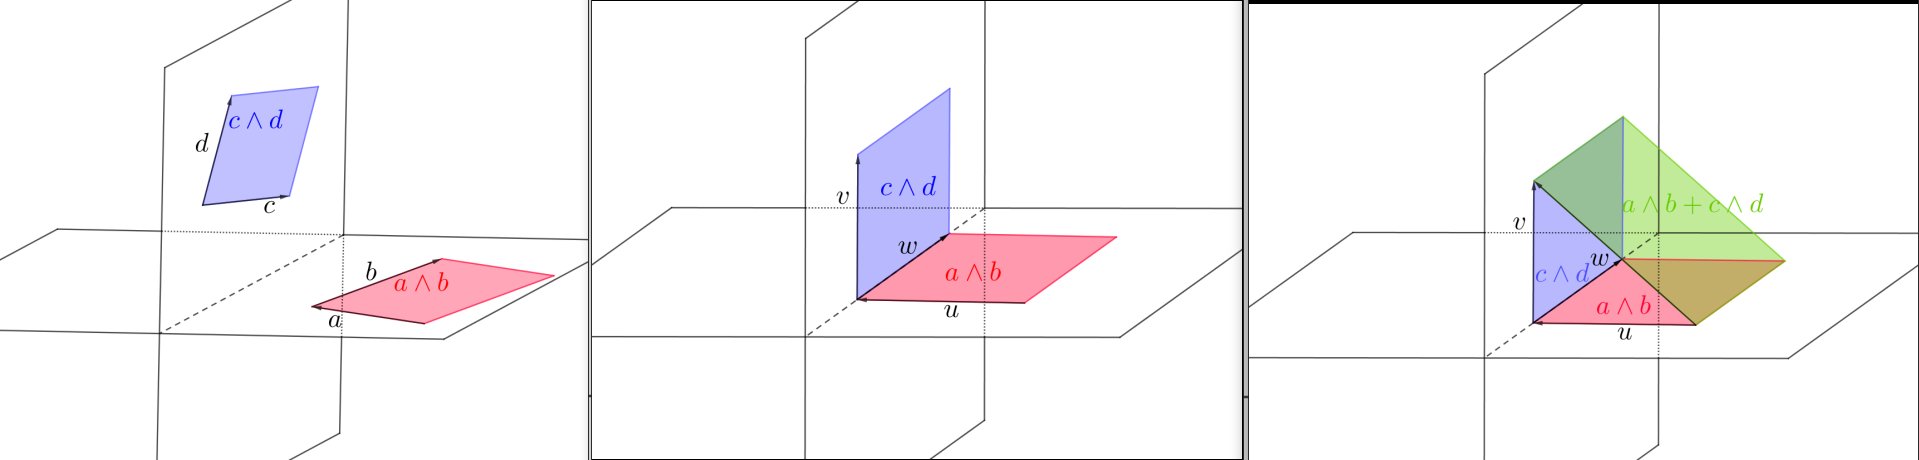
\includegraphics[scale=0.25]{sommebivecteurs.png}
\caption{L'addition de deux bivecteurs}
\label{sommebivecteurs}
\end{figure}


\subsubsection{Lames et multivecteurs}

On peut continuer le même genre de constructions pour construire des trivecteurs $\bm{a} \wedge \bm{b} \wedge \bm{c}$, où les trois vecteurs $\bm{a}$, $\bm{b}$ et $\bm{c}$ ne sont pas coplanaires. Dans ce cas, le trivecteur représentera un espace de dimension 3 avec une orientation et une norme qui correspondra au volume du parallélépipède engendré par les trois vecteurs, comme sur la figure ci-dessous : 

\begin{figure}[!ht]
\centering
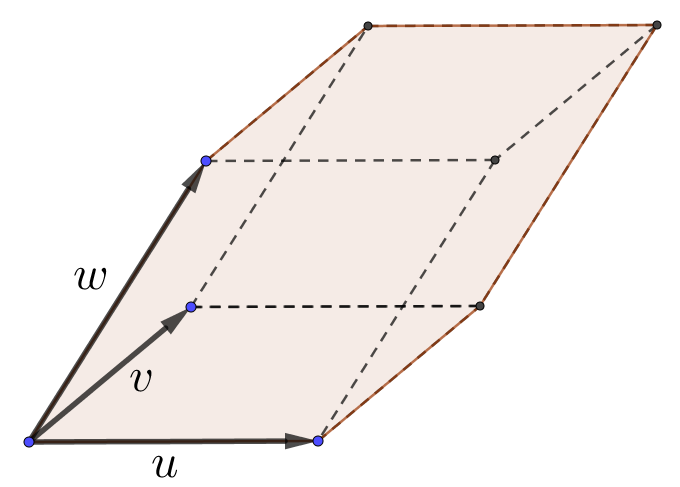
\includegraphics[scale=0.25]{trivecteur.png}
\caption{Un trivecteur}
\label{trivecteur}
\end{figure}

Plus généralement, ces objets sont appelés des lames : Une \sg{k-lame} (ou lame de \sg{grade} k) est un multivecteur $\bm{A}$ de la forme $$\bm{A} = \bm{a_1}  \wedge \bm{a_2} \wedge \cdots \wedge \bm{a_k}$$ où les vecteurs  $\bm{a_1}, \cdots \bm{a_k}$ sont linéairement indépendants. 


Les 0-lames sont les constantes réelles, les 1-lames les vecteurs, les bivecteurs sont les 2-lames, les trivecteurs les 3-lames... 

Le grade maximal est $n$ : il n'y a qu'une $n$-lame (à une constante près) : $\bm{e_1} \wedge \cdots \wedge \bm{e_n}$. Cette lame est notée $I$ et est appelée \sg{pseudo-scalaire}.

Un multivecteur sous sa forme générale est donc une somme de lames de grades différents. Par exemple, dans $\mathscr{G}^3$, $2+ \bm{e_1}-3\bm{e_3}+2e_{12}-4e_{123}$ est un multivecteur.

Les lames et multivecteurs seront notés avec une lettre majuscule et les lames seront notées en gras.  

\subsubsection{Réversion et inverse}

Pour une $k$-lame $\bm{A} = \bm{a_1} \wedge \cdots \wedge \bm{a_k}$, on appelle réversion de $\bm{A}$, et on note $\bm{\tilde{A}}$ la lame $\bm{\tilde{A}} = \bm{a_k} \wedge \cdots \wedge \bm{a_1}$.

Pour une lame non nulle $\tilde{\bm{A}}$, le calcul de $\tilde{\bm{A}}$ donne : $\tilde{\bm{A}} =  \bm{a_k} \wedge \cdots \wedge \bm{a_1} = (-1)^{\frac{k(k-1)}{2}}\bm{A}$ car le produit extérieur est anti-commutatif sur les vecteurs de la base et on effectue $1+2+\cdots +(k-1)$ inversions pour passer de $\tilde{\bm{A}}$ à $\bm{A}$.

Donc on trouve : $\bm{A}\tilde{\bm{A}} = (-1)^{\frac{k(k-1)}{2}}\bm{A}^2 = (-1)^{\frac{k(k-1)}{2}}||\bm{A}||^2$, d'où les lames sont inversibles et  $$\bm{A}^{-1} = \frac{(-1)^{\frac{k(k-1)}{2}}}{||\bm{A}||^2} \tilde{\bm{A}}$$

En particulier, les vecteurs ont donc un inverse et on a : $\bm{u}^{-1} = \frac{\bm{u}}{||\bm{u}||^2}$. 

Mais les multivecteurs en général n'ont pas d'inverse, l'algèbre n'est donc pas un corps.

\subsubsection{Dual d'un multivecteur}

Rappelons la définition du pseudo-scalaire : $\bm{I} = \bm{e_1} \wedge \cdots \wedge \bm{e_n}$.  Donc $\bm{I}$ est inversible et $\bm{I}^{-1} = \pm \bm{I}$ selon la valeur de $n$. 

Le \sg{dual} d'un multivecteur $A$ est le multivecteur noté $A^*$ et égal à $A^* = A\bm{I^{-1}}$.

Géométriquement, on peut imaginer le dual d'un multivecteur comme tout l'espace n'étant pas engendré par ce multivecteur. Par exemple, dans $\mathscr{G}^3$, on a $\bm{I^{-1}} = -\bm{e_1} \wedge \bm{e_2} \wedge \bm{e_3}$, et donc on a : $\bm{e_{1}}^* = -\bm{e_1}\wedge \bm{e_1}\wedge \bm{e_2} \wedge \bm{e_3} = -\bm{e_2} \wedge \bm{e_3}$.

Une lame de grade $k$ aura donc un dual de grade $n-k$. 

\subsection{Algèbre géométrique conforme (CGA)}

\subsubsection{Présentation}
Dans tout ce que nous venons de voir précédemment, nous étions dans l'espace vectoriel euclidien $\R^3$, tous les objets comme les droites et les plans passaient par l'origine. Pour pouvoir traiter tous les objets de l'espace affine, ainsi que d'autres comme les sphères et les cercles, nous allons nous placer dans une algèbre géométrique bien particulière : \sg{l'algèbre géométrique conforme}, abrégée \sg{CGA} (pour Conformal Geometric Algebra).

Pour construire une telle algèbre, notée $\mathscr{G}^{4,1}$, nous allons prendre un espace de dimension 5. Une base orthogonale des vecteurs de $\mathscr{G}^{4,1}$ est constituée des trois premiers vecteurs de base de $\R^3$ : $\bm{e_1}$, $\bm{e_2} $, et $\bm{e_3}$ , ainsi que de deux vecteurs supplémentaires, notés $\bm{e_+}$ et $\bm{e_-}$ avec les conventions suivantes : 
$$||\bm{e_+}|| = 1 \text{ et } ||\bm{e_-}|| = -1$$ 

En pratique, on utilisera plutôt les vecteurs $\bm{e_0}$ et $\ei$ définis par : 
$$ \bm{e_0} = \frac{1}{2} (\bm{e_-} - \bm{e_+}) \text{ et }  \ei = \bm{e_+}+ \bm{e_-}$$
de telle sorte que : 
\begin{eqnarray}
&\bullet & ||\ez||=||\ei|| = 0 \label{normeezei}\\
&\bullet &\ez \wedge \ei = -\e{+} \wedge \e{-}\\
&\bullet &\ez \cdot \ei = \ei \cdot \ez = -1 \label{ezei}\\
&\bullet &\text{Pour } k\in \lbrace1,2,3\rbrace \text{, }\ez \cdot \e{k} = \ei \cdot \e{k} = 0 \label{psbase}
\end{eqnarray}

\subsubsection{Image d'un point en CGA}

Dans toute la suite, on notera en gras $\bm{x}$ le vecteur de $\R^3$ et $x$ le même vecteur dans le système de coordonnées CGA.

A $\bm{x}$ de coordonnées $(a,b,c)$ dans une base donnée de $\R^3$, on associe le vecteur CGA par la formule : $x = a \bm{e_1} + b \bm{e_2} + c \bm{e_3} + \bm{e_0} + \frac{1}{2}||\bm{x}||^2 \ei$, ce qui s'écrit aussi : 

$$x = \bm{x} + \bm{e_0} + \frac{1}{2}||\bm{x}||^2 \ei$$

De cette manière-là, pour un autre point $y$, on obtient : 

\begin{eqnarray*}
x \cdot y & = &  \left(\bm{x} + \bm{e_0} + \frac{1}{2}||\bm{x}||^2 \ei\right) \cdot  \left(\bm{y} + \bm{e_0} + \frac{1}{2}||\bm{y}||^2 \ei\right) \\
& = & \bm{x} \cdot \bm{y} +  \frac{1}{2}||\bm{y}||^2 \ez \cdot \ei +  \frac{1}{2}||\bm{x}||^2 \ei \cdot \ez \text{ car les autres termes s'annulent d'après }\ref{normeezei}\text{ et } \ref{psbase} \\
& = & \bm{x} \cdot \bm{y} -  \frac{1}{2}\bm{y}^2 -  \frac{1}{2}\bm{x}^2 \text{ d'après }\ref{ezei} \\
& = & - \frac{1}{2} \left( \bm{x}^2 -2 \bm{x} \cdot \bm{y} + \bm{y}^2\right)  \\
\end{eqnarray*}
et finalement : 
$$ x \cdot y =  - \frac{1}{2} ||\bm{x}-\bm{y}||^2$$

On remarque alors que le produit scalaire entre deux points est proportionnel à la distance au carré entre ces deux points, ce qui nous permet tout de suite de définir les points en CGA comme étant les vecteurs de norme nulle.
 
\subsubsection{Normalisation}

A un point CGA $x = \bm{x} + a \bm{e_0} + b \ei$, on remarque que $-\ei \cdot x = a$ d'après les propriétés précédentes. On obtient ainsi un procédé de "normalisation", similaire à ce qui se fait en géométrie projective : 

Si $a\neq 0$, le vecteur $\frac{x}{-\ei \cdot x}$ a pour coefficient $1$ devant $\ez$, et donc les coordonnées du point correspondant se lisent devant $\eu$, $\ed$ et $\et$.

Un point CGA possède donc en prime un "poids", égal à $-\ei \cdot x$. 

On remarque également que l'image de l'origine est $\ez$, ce vecteur représente donc l'origine du repère en CGA (d'où la notation).

Aussi, le vecteur $\ei$ peut être vu comme un point à l'infini : si on divise $\bm{x}$ par la constante $-\bm{x} \cdot \ez = \frac{1}{2}\bm{x}^2$, (donc le même point, au poids près) on trouve :

\begin{eqnarray*}
\frac{\bm{x}}{-\bm{x} \cdot \ez} &=& \frac{2}{\bm{x}^2} \left( \bm{x} +\ez + \frac{1}{2}\bm{x}^2 \ei\right)\\
 &=& 2 \left( \frac{1}{\bm{x}} + \frac{1}{2}\ei + \frac{\ez}{\bm{x}^2} \right) \xrightarrow[\bm{x}\rightarrow \infty]{} \ei\\
\end{eqnarray*}

\subsubsection{Objets géométriques en CGA - Représentations IPNS et OPNS}

La force des algèbres géométriques est qu'avec elles, on peut représenter non seulement les points, mais aussi d'autres lieux géométriques de $\R^3$ comme des sphères, des plans, des droites, et des cercles toujours avec des multivecteurs. En fait, il existe même deux représentations différentes pour chaque objet $E$ : l'IPNS et l'OPNS (Inner et Outer Product Null Space).

\begin{itemize}
\item l'IPNS consiste à dire que le multivecteur $x$ correspond à notre espace $E$ si $$\forall y \text{ vecteur de } \mathscr{G}^{4,1}, y\in E \Leftrightarrow x \cdot y =0.$$
\item l'OPNS consiste à dire que le multivecteur $x$ correspond à notre espace $E$ si $$\forall y \text{ vecteur de } \mathscr{G}^{4,1}, y\in E \Leftrightarrow x \wedge y =0.$$
\end{itemize}

Ces deux représentations sont duales l'une de l'autre. En effet, on a la formule (qui ne sera pas démontrée ici) $$a \cdot b = (a \wedge b^*)^*$$ 
Donc $a \cdot b =0 \Longleftrightarrow a \wedge b^*=0$. 

On peut donc facilement passer d'une représentation à une autre. 

On obtient le tableau suivant :\vspace*{0.3cm}

\begin{table}[h!]
\begin{center}
\hspace*{-2.5cm} 
\begin{tabular}{|c|c|c|c|c|c|}
\hline

Objets & Caractéristiques & Représentation IPNS & Grade & Représentation OPNS & Grade \\\hline
Point $x$ & $\bm{x}$ : coordonnées dans  $\R^3$  & $x = \bm{x} + \bm{e_0} + \frac{1}{2}||\bm{x}||^2 \ei$ & 1 & $x^* = s_1 \wedge s_2 \wedge s_3 \wedge s_4$ & 4 \\
& $s_1, s_2, s_3, s_4$ : sphères contenant $x$& & & &\\
\hline

Sphère $s$ &  $\bm{c}$ : coordonnées du centre  & $s = \bm{c} + \frac{1}{2}(\bm{c}^2-r^2)\ei + \ez$ & 1 & $s^* = a \wedge b \wedge c \wedge d$ & 4 \\
& $r$ : rayon & & & &\\
& $a, b, c, d$ : points sur $s$ & & & &\\\hline

Plan $P$ &  $\bm{n}$ : vecteur normal à $P$  & $P = \bm{n} + d\ei$ & 1 & $P^* = a \wedge b \wedge c \wedge \ei$ & 4 \\
& $d$ : distance de $P$ à l'origine & & & &\\
& $a, b, c$ : points sur $P$ & & & &\\\hline

Droite $D$  &  $P_1, P_2$ : plans contenant $D$  & $D = P_1 \wedge P_2$ & 2 & $D^* = a \wedge b \wedge \ei$ & 3 \\
& $a, b$ : points sur $D$ & & & &\\\hline

Cercle $c$ &  $s_1, s_2$ : sphères contenant $c$  & $c = s_1 \wedge s_2$ & 2 & $c^* = a \wedge b \wedge c$ & 3 \\
& $a, b, c$ : points sur $P$ & & & &\\\hline

Paire de  &  $s_1, s_2, s_3$ : sphères contenant $P_p$  & $P_p = s_1 \wedge s_2 \wedge s_3 $ & 3 & $P_p^* = a \wedge b$ & 2 \\
points $P_p$ & $a, b$ : points de $P_p$ & & & &\\\hline
\end{tabular}
\end{center}
\caption{Tableau des représentation IPNS et OPNS des objets géométriques classiques}
\renewcommand{\thetable}{\arabic{table}}
\label{tableau}
\end{table}

\newpage
Une paire de points représente, en un multivecteur, deux points. 

\subsubsection{Transformations : réflexions, rotations et translations}
\label{transformations}
 Soient $\bm{a}$ et $\bm{x}$ deux vecteurs. Comme vu auparavant, $\bm{a}$ est donc inversible et $\bm{a}^{-1} = \frac{\bm{a}}{\bm{a^2}}$. Donc : 
\begin{equation*}
\bm{x} = \bm{x a a}^{-1} = (\bm{xa})\bm{a}^{-1}= (\bm{x}\cdot \bm{a} + \bm{x} \wedge \bm{a})\bm{a}^{-1} = (\bm{x}\cdot \bm{a})\bm{a}^{-1} + (\bm{x} \wedge \bm{a})\bm{a}^{-1}
\end{equation*}

On va à présent montrer que l'égalité 
\begin{equation}
\bm{x} =  (\bm{x}\cdot \bm{a})\bm{a}^{-1} + (\bm{x} \wedge \bm{a})\bm{a}^{-1}\label{decomp}
\end{equation}
représente la décomposition orthogonale de $\bm{x}$ selon le vecteur $\bm{a}$ : 

On remarque déjà que $(\bm{x}\cdot \bm{a})\bm{a}^{-1} = \frac{\bm{x}\cdot \bm{a}}{\bm{a}^2}\bm{a}$, donc est bien colinéaire à $\bm{a}$.

Montrons à présent que $(\bm{x}\wedge \bm{a})\bm{a}^{-1}$ est orthogonal à $\bm{a}$, c'est-à-dire que $(\bm{x}\wedge \bm{a})\bm{a}^{-1} \cdot \bm{a} = 0 $: 

\begin{eqnarray*}
(\bm{x}\wedge \bm{a})\bm{a}^{-1} \cdot \bm{a} &=&  ((\bm{x}\bm{a}-\bm{x}\cdot \bm{a} )\bm{a}^{-1}) \cdot \bm{a}  \text{ d'après la formule fondamentale}\\
&=&  (\bm{x}\bm{a}\bm{a}^{-1}) \cdot \bm{a}-((\bm{x}\cdot \bm{a})\bm{a}^{-1}) \cdot \bm{a} \text{ en développant}\\
&=&  \bm{x} \cdot \bm{a}-(\bm{x}\cdot \bm{a})(\bm{a}^{-1} \cdot \bm{a}) \text{ car } \bm{x}\cdot \bm{a} \text{ est une constante }\\
&=&  \bm{x} \cdot \bm{a}-(\bm{x}\cdot \bm{a})(\frac{\bm{a}}{\bm{a}^2}\cdot \bm{a}) \\
&=&  \bm{x} \cdot \bm{a}-\bm{x}\cdot \bm{a}\\
&=&  0
\end{eqnarray*}

On a donc bien démontré que la décomposition de $\bm{x}$ donnée en \ref{decomp} est la décomposition orthogonale selon $\bm{a}$.

A présent, calculons $\bm{axa}^{-1}$ : 

$$ \bm{axa}^{-1} = (\bm{ax})\bm{a}^{-1} = (\bm{a}\cdot \bm{x})\bm{a}^{-1}+(\bm{a}\wedge \bm{x})\bm{a}^{-1} = (\bm{x}\cdot \bm{a})\bm{a}^{-1}-(\bm{x}\wedge \bm{a})\bm{a}^{-1} $$

On remarque qu'il s'agit de la même décomposition qu'en \ref{decomp}, mais avec le signe qui a changé. Le vecteur $\bm{axa}^{-1}$ représente donc la réflexion de $\bm{x}$ par rapport au vecteur $\bm{a}$, comme illustré sur le dessin ci-dessous : 

\begin{figure}[!ht]
\centering
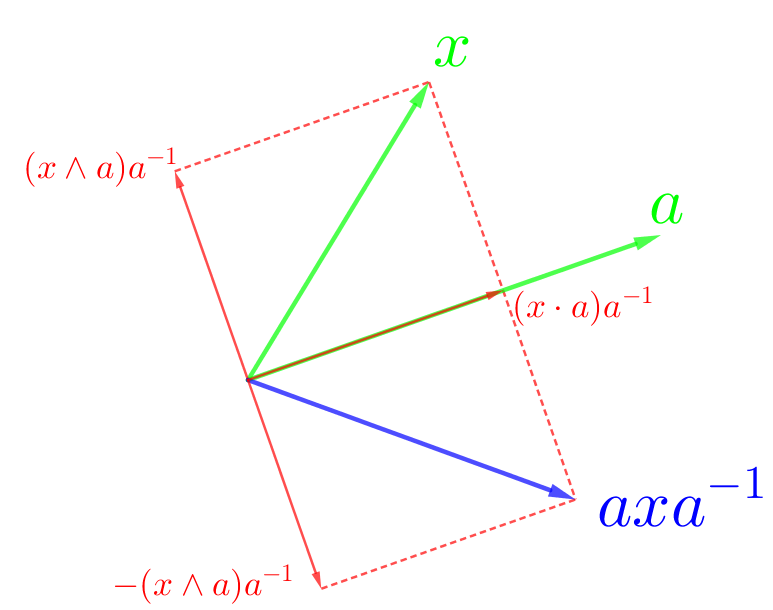
\includegraphics[scale=0.3]{reflexion.png}
\caption{Réflexion de $\bm{x}$ par rapport au vecteur $\bm{a}$}
\label{reflexion}
\end{figure}

Cette opération (appelée le \sg{sandwich}) est assez pratique pour faire les calculs : par exemple pour composer deux réflexions (selon $\bm{a}$ et $\bm{b}$), il suffit de "sandwicher" deux fois : $\bm{baxa}^{-1}\bm{b}^{-1}$. Mais comme ce vecteur est aussi égal à $(\bm{ba})\bm{x}(\bm{ba})^{-1}$, on peut représenter cette transformation par un seul multivecteur, $\bm{ba}$.

En pratique, on va également choisir les vecteurs $\bm{a}$ et $\bm{b}$ unitaires de sorte que $\bm{a}^{-1}=\bm{a}$ et $\bm{b}^{-1}=\bm{b}$. Ainsi l'inverse de $\bm{ba}$ sera $\tilde{\bm{ba}} = \bm{ab}$

Comme toute rotation et toute translation est la composée de deux réflexions, on peut ainsi définir des multivecteurs représentant ces transformations et les "sandwicher" au multivecteur qu'on souhaite transformer. 

En pratique, les formules (non démontrées ici, se référer à \cite{Dorst}) sont : 
\begin{itemize}
\item Pour une rotation d'angle $\theta$ de plan ayant $\bm{n}$ comme vecteur normal, on note $$R = cos\left(\frac{\theta}{2}\right)- sin\left(\frac{\theta}{2}\right) \bm{n}$$ (appelé \sg{rotor}). L'image du multivecteur $X$ par cette rotation est $RX\tilde{R}$.
\item Pour une translation de vecteur $\bm{t}$, on note $$T = 1-\frac{1}{2} \bm{t} \ei $$ L'image du multivecteur $X$ par cette translation est $TX\tilde{T}$.
\end{itemize}

\section{L'assistant de preuve Coq}

\subsection{Présentation}

Coq est un logiciel assistant de preuve développé par l'INRIA et basé sur le langage Gallina. Un assistant de preuve est un logiciel permettant de faire des démonstrations mathématiques afin de prouver des assertions. Pour cela, il faut d'abord formuler le théorème à démontrer, puis le démontrer à l'aide de "tactiques" qui sont des instructions de modification de la preuve. 

Un des plus grands tours de force de ce logiciel a été de démontrer formellement le théorème de Feit-Thompson (tout groupe fini d'ordre impair est résoluble) dont la démonstration initiale faisait 250 pages. Il a fallu cependant une équipe d'une dizaine de chercheurs qui ont travaillé à temps plein pendant 6 ans afin d'aboutir à ce résultat. On voit donc que la mécanisation de la démonstration d'un théorème peut être très longue. De même, vérifier la validité d'un algorithme prend en général bien plus de temps que de trouver l'algorithme lui-même.

\subsection{Exemple}

Le plus simple est de visualiser un exemple. Prouvons la formule bien connue : $$\forall n\in \N, \sum_{k=0}^n = \frac{n(n+1)}{2}$$

Premièrement, il nous faut définir la somme des $n$ premiers entiers. Coq utilise un langage de programmation fonctionnel, c'est-à-dire que tout ce que nous manipulons est fonction. Les définitions se font donc de façon récursive. Voici la définition : 

\begin{figure}[!ht]
\centering
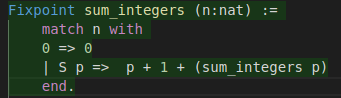
\includegraphics[scale=0.6]{coq1.png}
\caption{Définition de la somme des n premiers entiers}
\end{figure}

Le mot-clé "Fixpoint" permet de définir des objets de façon récursive, on précise que $n$ est de type entier naturel (nat). 

En Coq, les entiers sont également codés de façon récursive de la façon suivante : tout entier naturel $n$ est soit $0$, soit il existe un entier naturel noté $p$ tel que $n = S\ p$, où $S$ est la fonction successeur. Avec cette notation, on doit donc séparer deux cas : soit $n$ vaut $0$, et alors la réponse est $0$, soit $n$ s'écrit $S\ p$ et dans ce cas-là, la somme des $n$ premiers entiers est celle jusqu'à $p$ et $p+1$.

On vérifie que notre fonction calcule bien la somme en testant la somme des cinq premiers entiers : 
\begin{figure}[!ht]
\centering
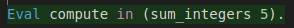
\includegraphics[scale=0.6]{coq2.png}
\end{figure}
\begin{figure}[!ht]
\centering
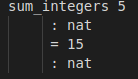
\includegraphics[scale=0.6]{coq3.png}
\end{figure}

Le résultat a donc l'air correct. On peut maintenant définir notre théorème : 

\begin{figure}[!ht]
\centering
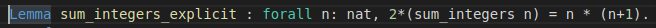
\includegraphics[scale=0.6]{coq4.png}
\caption{Théorème à démontrer}
\end{figure}
\newpage
On évite, pour des raisons de divisions dans les entiers naturels d'exprimer directement le théorème. En effet, celui-ci implique que la valeur $n(n+1)$ est divisible par $2$, ce qui est vrai, mais non prouvé, et donc à faire en Coq. On voit alors dans une fenêtre à droite qu'il reste une proposition à démontrer (le theorème lui-même) : 

\begin{figure}[!ht]
\centering
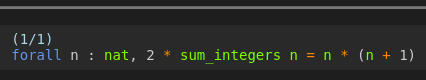
\includegraphics[scale=0.6]{coq5.png}
\end{figure}

 Pour le démontrer, nous allons appliquer différentes tactiques, la plupart du temps similaire à ce que nous ferions sur une feuille de papier. Ici, la proposition commence par un $\forall$, donc on aimerait écrire "Soit $n\in \N$", ce qui se fait avec la tactique "intros" : 
\begin{figure}[!ht]
\centering
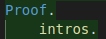
\includegraphics[scale=0.6]{coq6.png}
\end{figure}

On voit alors que la fenêtre des propriétés à démontrer est modifiée : en-haut de la barre, les hypothèses ($n$ est entier naturel) et en-dessous, ce qu'il reste à démontrer :

\begin{figure}[!ht]
\centering
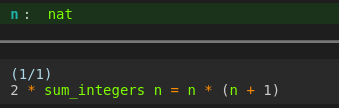
\includegraphics[scale=0.6]{coq7.png}
\end{figure}

On veut raisonner par récurrence sur $n$, ce qui s'écrit : 

\begin{figure}[!ht]
\centering
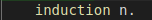
\includegraphics[scale=0.6]{coq8.png}
\end{figure}

La fenêtre de démonstration nous dit cette fois-ci qu'il y a deux propositions à démontrer. On commence par le théorème pour $n=0$, puis le théorème pour $n+1$ sachant celui-ci vrai pour $n$.
 
L'initialisation est très simple à montrer, il ne s'agit que d'un simple calcul, on peut utiliser pour cela la tactique "intuition". La fenêtre de démonstration devient :
\begin{figure}[!ht]
\centering
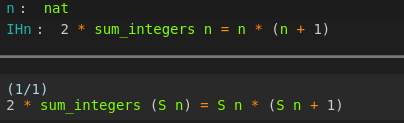
\includegraphics[scale=0.6]{coq10.png}
\end{figure}

Il ne reste plus qu'une proposition à démontrer, et pour celle-ci, les hypothèses sont que $n$ est entier naturel et que la propriété est vraie au rang $n$. On utilise la tactique "simpl" pour simplifier la proposition, c'est-à-dire que Coq va remplacer "sum\_integers (S n)" par sa définition : "n+1+sum\_integers n" : 

\begin{figure}[!ht]
\centering
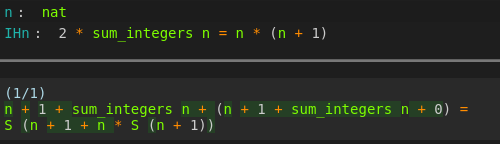
\includegraphics[scale=0.6]{coq11.png}
\end{figure}

Ensuite, les trois tactiques suivantes vont chercher des propriétés déjà connues par la bibliothèque de Coq : 
\begin{figure}[!ht]
\centering
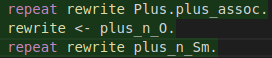
\includegraphics[scale=0.6]{coq12.png}
\end{figure}

Ici, l'associativité de l'addition, le fait que $n+0=n$, et une formule sur $S (n+m)$. La tactique "repeat" permet d'utiliser plusieurs fois la tactique qui suit.  On obtient :
\begin{figure}[!ht]
\centering
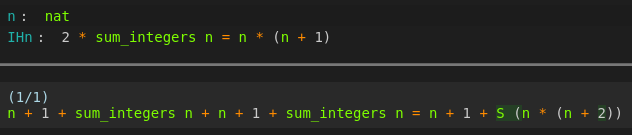
\includegraphics[scale=0.6]{coq13.png}
\end{figure}

On simplifie ce qui est trouvé à l'aide de la tactique "ring\_simplify", et on obtient :\newpage
\begin{figure}[!ht]
\centering
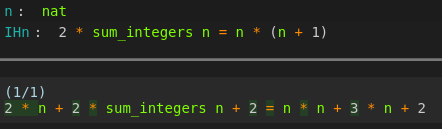
\includegraphics[scale=0.6]{coq14.png}
\end{figure}

On peut maintenant appliquer l'hypothèse de récurrence grâce à la tactique 

\begin{figure}[!ht]
\centering
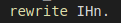
\includegraphics[scale=0.6]{coq15.png}
\end{figure}

qui donne

 \begin{figure}[!ht]
\centering
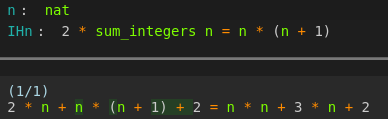
\includegraphics[scale=0.6]{coq16.png}
\end{figure}

Enfin, il ne reste plus qu'un calcul, qu'on vérifie grâce à la tactique "ring", et à la fin est affiché : 
\begin{figure}[!ht]
\centering

\includegraphics[scale=0.6]{coq17.png}
\end{figure}

Le théorème est donc entièrement prouvé :

\begin{figure}[!ht]
\centering
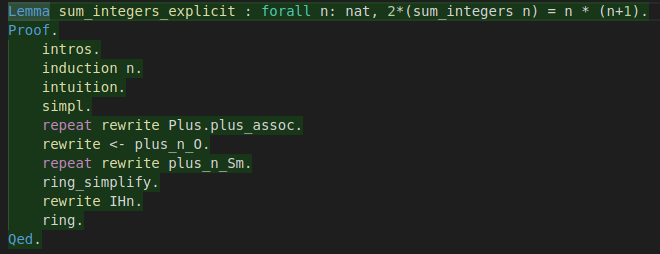
\includegraphics[scale=0.6]{coq18.png}
\caption{Démonstration complète de la formule en Coq}
\end{figure}

On pourra donc le réutiliser par la suite dans d'autres démonstrations.


\section{Implémentation de mouvements de robots à l'aide des algèbres géométriques en Coq}

Dans cette partie, nous allons implémenter en Coq les différentes formules de CGA vues au deuxième paragraphe (les différentes représentations IPNS et OPNS), nous prouverons que cela donne bien ce qui est attendu (la formule d'un cercle donne bien un cercle...). Nous constaterons ensuite sur le logiciel CLUCalc (qui est un outil  de visualisation 3D des algèbres géométriques) que ce qui a été implémenté en Coq donne bien ce qui est attendu graphiquement pour trois robots donnés. 

\subsection{Algèbres Géométriques Conformes}

Tout d'abord, nous réutiliserons la bibliothèque de Laurent Théry \cite{Thery}, qui a déjà implémenté les algèbres géométriques en Coq. Nous spécialisons cette librairie pour n'utiliser que des algèbres géométriques conformes. On donne donc la dimension égale à 5. La classe \textit{vect} contiendra les multivecteurs en général et la classe \textit{point} contiendra les points de $\R^3$. 
\begin{figure}[!ht]
\centering
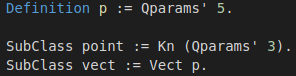
\includegraphics[scale=0.6]{cga1.png}
\end{figure}

Après plusieurs vérifications de propriétés de base sur le produit extérieur, le produit scalaire et le produit géométrique, on implémente la formule d'un point en CGA, ainsi que les différents objets géométriques du tableau \ref{tableau}.\newpage

\begin{figure}[!ht]
\centering
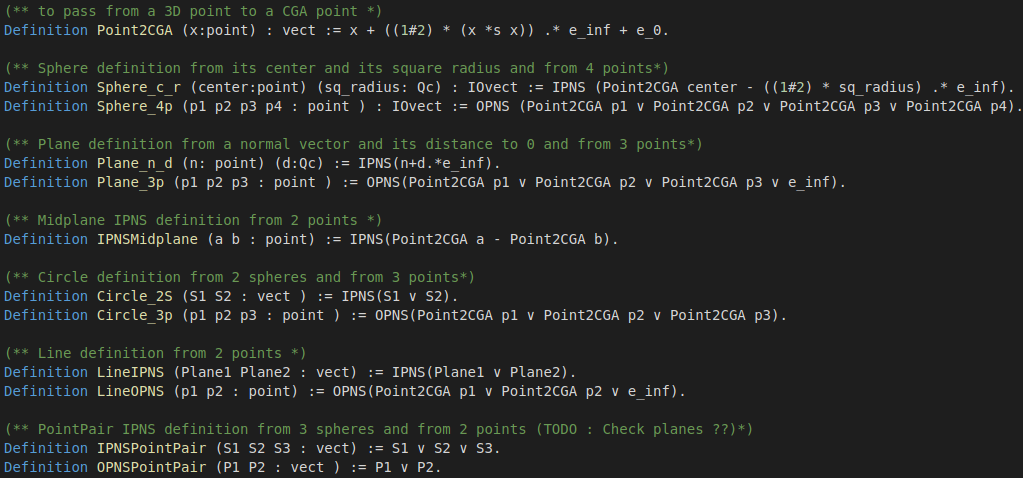
\includegraphics[scale=0.45]{cga2.png}
\caption{Implémentation du tableau \ref{tableau} en Coq}
\end{figure}

On a choisi de donner un "flag" IPNS ou OPNS à chaque multivecteur. En effet, ce typage aidera à savoir si l'objet géométrique représenté doit être considéré comme une représentation IPNS ou OPNS. Ensuite, on définit la fonction "is\_on\_object" qui dit si oui ou non un point est sur l'objet considéré :  

\begin{figure}[!ht]
\centering
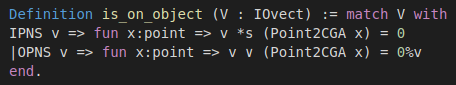
\includegraphics[scale=0.45]{cga3.png}
\end{figure}

Et ensuite, on démontre plusieurs lemmes, comme par exemple celui-ci : 
\begin{figure}[!ht]
\centering
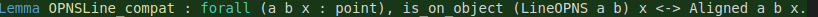
\includegraphics[scale=0.55]{cga4.png}
\end{figure}

On y dit que pour tout point $a$, $b$ et $x$, il est équivalent de dire que $x$ est sur l'objet défini par \textit{LineOPNS a b} (donc que $x\wedge (LineOPNS\ a\ b) = 0$) et que $a$, $b$ et $x$ sont alignés (la fonction \textit{Aligned} étant définie auparavant).

Ces démonstrations étant en général peu importantes dans les livres, elles n'y figurent pas toutes. Reconstruire la preuve en Coq permet donc de bien vérifier que ces théorèmes sont valides. L'idée générale de ces démonstrations est de remplacer les vecteurs par leur décomposition selon la base, de développer les calculs avec le produit extérieur, et de simplifier. Une démonstration à la main impliquerait peut-être une méthode différente, plus élégante, mais le fait d'utiliser un logiciel comme Coq permet de finalement simplifier la logique des démonstrations, ou tout du moins de laisser les calculs compliqués à la machine. 

\subsection{Cinématique directe}

Dans cette section-là, nous allons calculer la cinématique directe de différents robots. On ne considérera que des robots série, c'est-à-dire constitué d'une seule chaîne d'éléments ayant entre eux des liaisons soit glissière (translations) soit pivotantes (des rotations). La cinématique directe consiste à trouver la position et la direction du bout du robot (appelé \sg{effecteur}) étant donnés tous les paramètres nécessaires pour le calculer. En pratique, on se donne une position de référence, une longueur pour chaque liaison glissière et un angle pour chaque rotation.

On a vu dans le chapitre \ref{transformations} que pour appliquer une translation de vecteur $t$, il suffit de calculer $M =  1-\frac{1}{2}t\ei$, dans le cas d'une rotation de plan de vecteur normal $\bm{n}$ et d'angle $\theta$, de calculer $M=cos\left(\frac{\theta}{2}\right)-sin \left(\frac{\theta}{2}\right)\bm{n}$ et enfin, en notant $x$ le point auquel on applique la transformation, de calculer $Mx\tilde{M}$.

On obtient donc les lignes suivantes :

\begin{figure}[!ht]
\centering
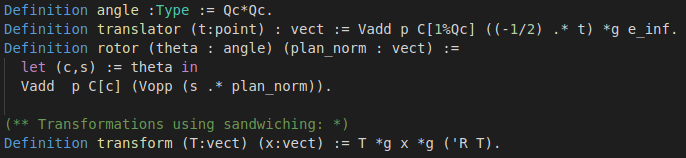
\includegraphics[scale=0.55]{robot1.png}
\caption{Définitions des angles, des translations et des rotations}
\end{figure}

Les réels étant assez compliqués à manipuler en Coq (car mathématiquement cet ensemble est compliqué, puisque c'est un ensemble de limites de suites de Cauchy), on a choisi ici de travailler dans le corps $\Q$. Un angle $\theta$ est donc représenté par le couple $(\cos(\theta), \sin(\theta))$ et les seuls angles considérés seront donc ceux dont ces valeurs seront rationnelles. En pratique, cela n'est pas très limitant car on peut montrer que tout angle réel peut être limite d'une suite d'angles ayant des cosinus et des sinus rationnels. Les robots étant des objets concrets, une approximation de chaque angle sera donc amplement suffisante.

\subsubsection{Robot RRP}

Le robot RRP est le robot possédant les liaisons schématiques suivantes : 

\begin{figure}[!ht]
\centering
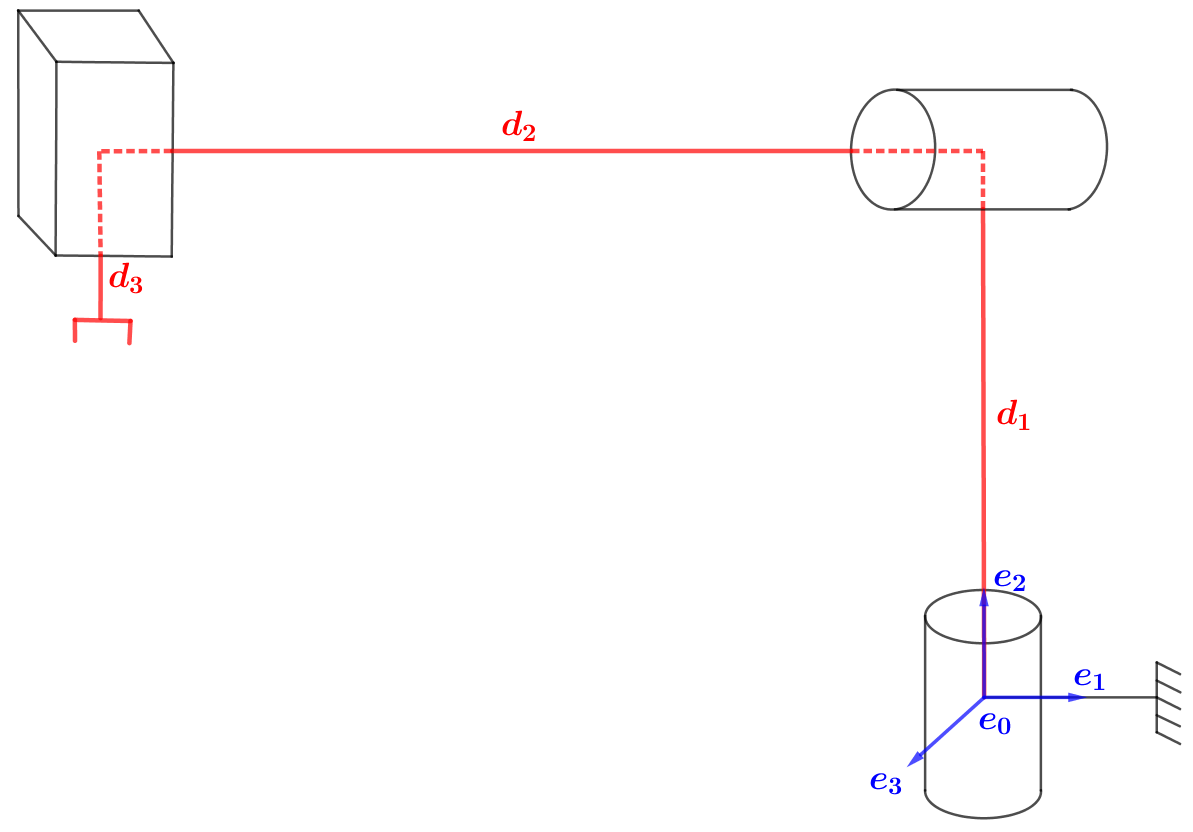
\includegraphics[scale=0.25]{RRP.png}
\caption{Schéma du robot RRP en configuration initiale}
\end{figure}

Il y a donc deux rotations, d'axe $\ed$ et d'axe $\eu$, et une translation d'axe $\ed$. 

En notant $d_i$ la longueur du bras $i$, pour $i\in \lbrace 1,2,3 \rbrace$, on obtient en Coq les définitions suivantes : 

\begin{figure}[!ht]
\centering
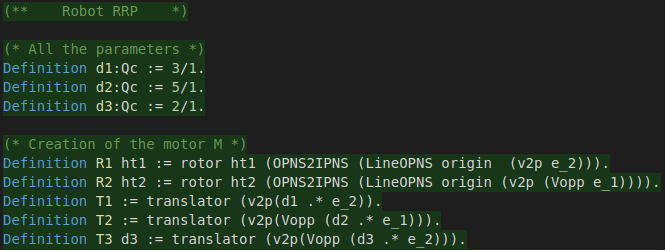
\includegraphics[scale=0.55]{RRPParametres.png}
\caption{Paramètres du robot RRP}
\end{figure}

$R1$ et $R2$ représentent les deux rotations, $T1$ et $T2$ les deux longueurs des deux premiers bras et $T3$ la longueur de la dernière translation (on remarque que $T3$ a un argument).

Le robot RRP est donc créé ainsi : 

\begin{figure}[!ht]
\centering
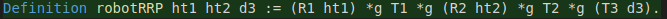
\includegraphics[scale=0.55]{RRPDef.png}
\caption{Définition du robot RRP}
\end{figure}

En rentrant les trois paramètres variables du robot, on obtient ainsi la position finale de l'effecteur. Testons ceci avec $d_3= 2$, $\theta_1 \approx 106.26 ^{\circ}$ et $\theta_2 \approx 134.76 ^{\circ}$. Ces angles ont été choisis car $\left(\cos \left(\frac{\theta_1}{2} \right), \sin \left(\frac{\theta_1}{2}) \right) \right) = \left(\frac{3}{5}, \frac{4}{5} \right) $ et $\left(\cos \left(\frac{\theta_2}{2} \right), \sin \left(\frac{\theta_2}{2} \right) \right) = \left(\frac{5}{13}, \frac{12}{13} \right) $. 

Voici le résultat obtenu (la fonction \textit{effector} renvoie l'image de l'origine par les transformations successives, donc la position finale de l'effecteur) : 

\begin{figure}[!ht]
\centering
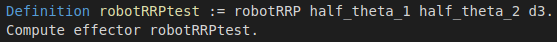
\includegraphics[scale=0.55]{RRPTest.png}

\caption{Test du robot RRP}
\end{figure}


\begin{figure}[!ht]
\centering
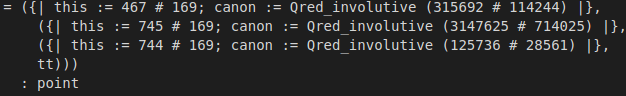
\includegraphics[scale=0.55]{RRPRes.png}
\caption{Position de l'effecteur du robot RRP pour notre test}
\end{figure}

Ceci signifie que l'effecteur a une position de coordonnées $\left( \frac{467}{169}, \frac{745}{169}, \frac{744}{169}  \right) \approx (2.76, 4.41, 4.40)$.

Vérifions cela. Nous allons utiliser le logiciel CLUCalc, avec lequel nous allons construire notre robot. Puis nous allons placer les angles des rotations et la longueur de la translation considérés et vérifier les résultats obtenus. Voici le robot obtenu : 
\newpage
\begin{figure}[!ht]
\centering
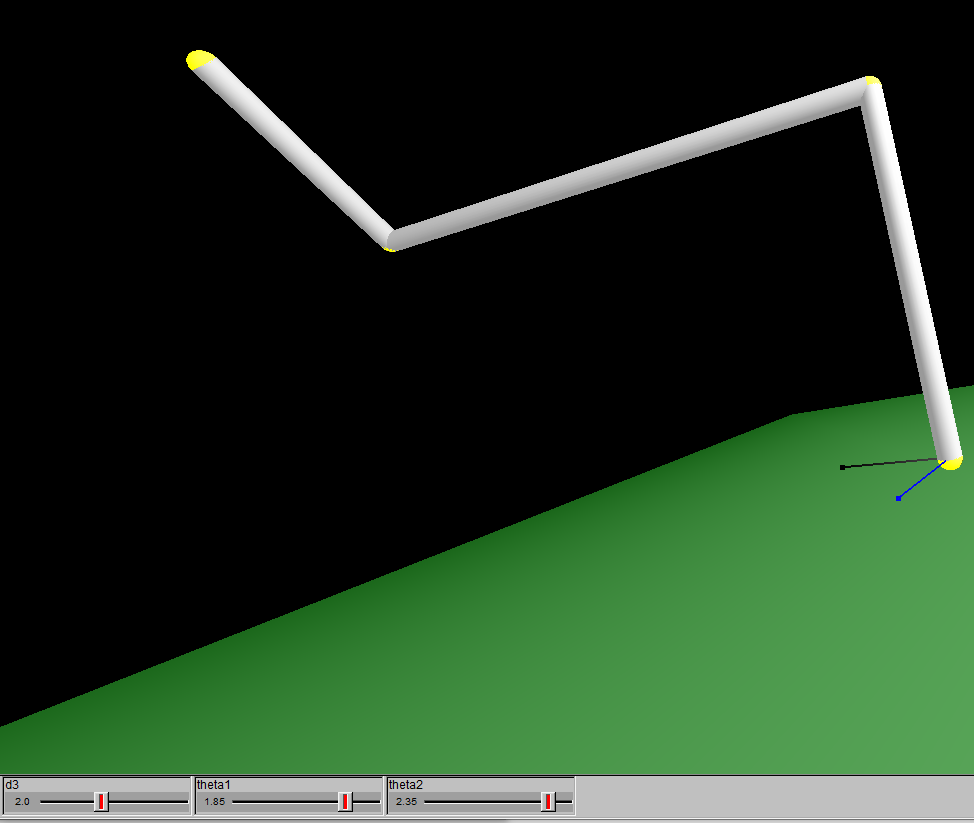
\includegraphics[scale=0.55]{RRPClucalc.png}
\caption{robot RRP construit en CLUCalc}
\end{figure}


En faisant afficher les coordonnées de la sphère finale (et de toutes les sphères intermédiaires), on peut en lire le centre en regardant les trois premières composantes. On s'aperçoit qu'il s'agit bien, aux arrondis près, des coordonnées trouvées en Coq : 

\begin{figure}[!ht]
\centering
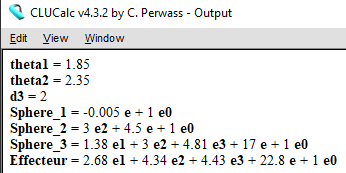
\includegraphics[scale=0.55]{RRPCluRes.png}
\caption{Position de l'effecteur du RRP en CLUCalc}
\end{figure}

\subsubsection{Robot SCARA }

Voici un exemple de robot SCARA, ainsi que ses liaisons schématiques : 

\begin{figure}[!ht]
    \begin{minipage}[c]{.46\linewidth}
        \centering
        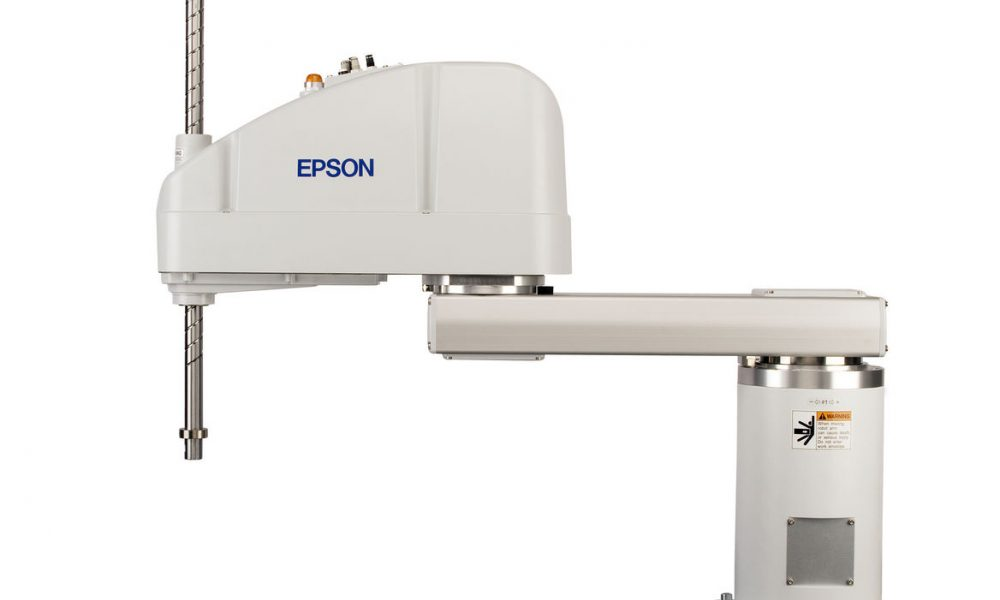
\includegraphics[scale=0.25]{Scara.jpg}
        \caption{Exemple de robot SCARA}
    \end{minipage}
    \hfill%
    \begin{minipage}[c]{.46\linewidth}
        \centering
        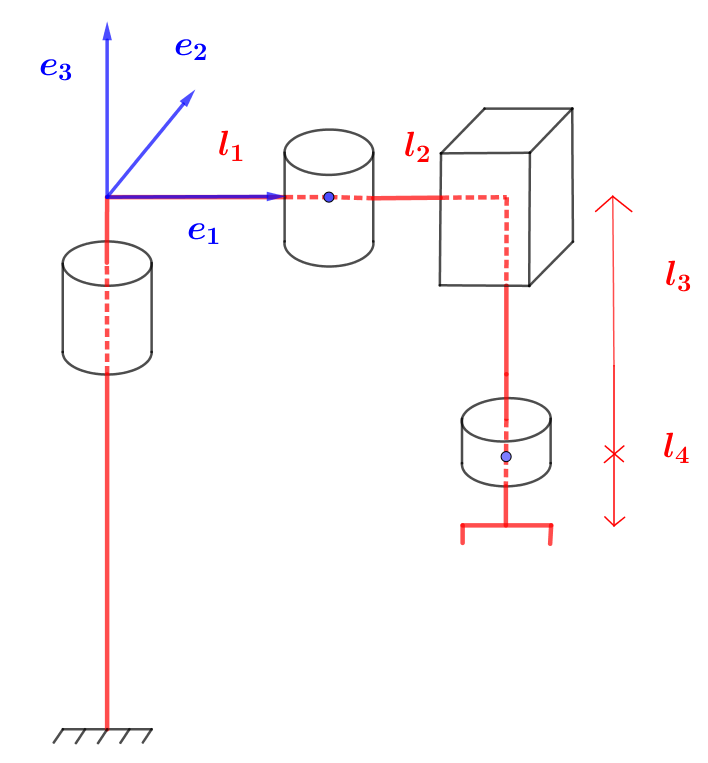
\includegraphics[scale=0.25]{Scara.png}
        \caption{Schéma du robot SCARA en configuration initiale}
    \end{minipage}
\end{figure}


Il y a donc trois bras, trois rotations de même axe $\et$ et une translation d'axe $\et$. 

En notant $l_i$ la longueur du bras $i$, pour $i\in \lbrace 1,2,3, 4 \rbrace$, on obtient en Coq les définitions suivantes : 

\begin{figure}[!ht]
\centering
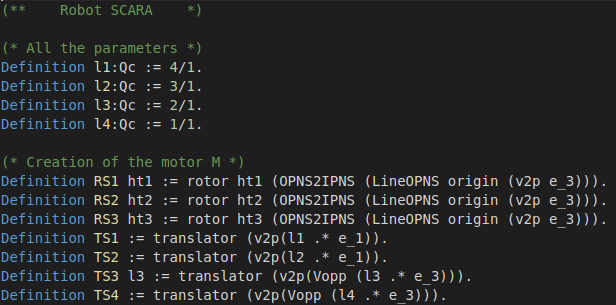
\includegraphics[scale=0.55]{SCARAParametres.png}
\caption{Paramètres du robot SCARA}
\end{figure}

$RS1$, $RS2$ et $RS3$ représentent les trois rotations, $TS1$, $TS2$ et $TS4$ les trois longueurs des bras et $TS3$ la longueur de la translation.

Le robot SCARA est donc créé et testé comme précédemment, avec des angles de $\theta_1 \approx 106.26 ^{\circ}$ et $\theta_2 \approx 134.76 ^{\circ}$. On rajoutera $\theta_3 \approx 123.86^\circ$ $\left( \text{car }\left(\cos \left(\frac{\theta_3}{2} \right), \sin \left(\frac{\theta_3}{2} \right) \right) = \left(\frac{8}{17}, \frac{15}{17} \right)\right) $. L'angle $\theta_4$ n'influe pas sur la position finale de l'effecteur (mais sur sa direction, ce qui est important si celui-ci n'est pas vu comme un point, mais comme un objet, par exemple une pince), on ne lui donne donc pas de valeur. 
\begin{figure}[!ht]
\centering
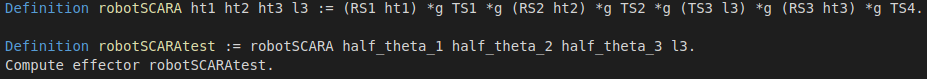
\includegraphics[scale=0.5]{SCARADef.png}
\caption{Définition et test du robot SCARA}
\end{figure}

On trouve : 

\begin{figure}[!ht]
\centering
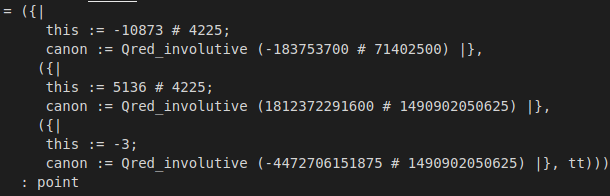
\includegraphics[scale=0.4]{SCARARes.png}
\caption{Résultat du test du robot SCARA}
\end{figure}

La position de l'effecteur est donc approximativement de $(-2.57, 1.22, -3)$.

Testons encore sur CLUCalc. Voici le robot avec la position testée : 

\begin{figure}[!ht]
\centering
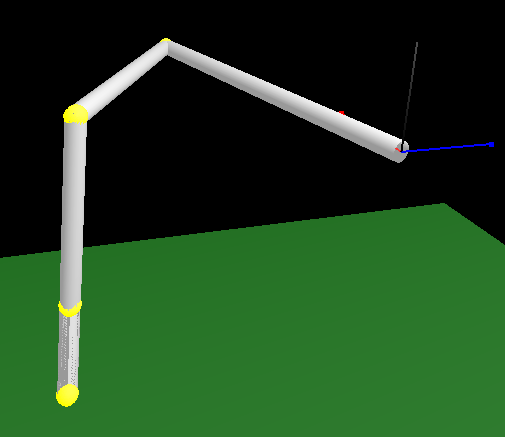
\includegraphics[scale=0.5]{SCARACluCalc.png}
\caption{robot SCARA construit en CLUCalc}
\end{figure}

Et la position finale de l'effecteur :

\begin{figure}[!ht]
\centering
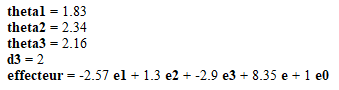
\includegraphics[scale=1]{SCARACluRes.png}
\caption{Position de l'effecteur du SCARA en CLUCalc}
\end{figure}

On voit que la position de l'effecteur $(-2.57,1.3,-2.9)$ est toujours correcte, aux arrondis près. 

\subsubsection{Robot 6R }

Un robot 6R est un robot ayant 6 axes de rotation. Il est constitué d'une base, ayant trois axes de rotation, et d'une partie plus petite appelée "poignet" avec trois autres axes de rotation, à l'extrémité du robot. En voici un exemple, avec les liaisons schématiques : 

\begin{figure}[!ht]
    \begin{minipage}[c]{.46\linewidth}
        \centering
        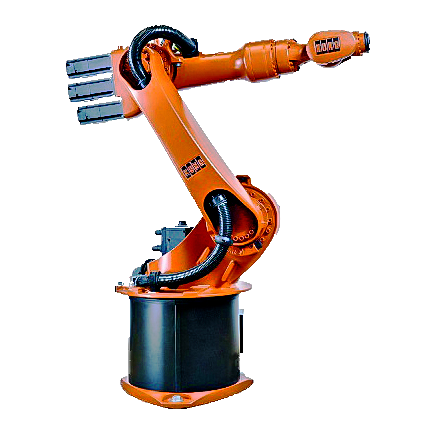
\includegraphics[scale=2]{6R.png}
        \caption{Un robot 6R}
    \end{minipage}
    \hfill%
    \begin{minipage}[c]{.46\linewidth}
        \centering
        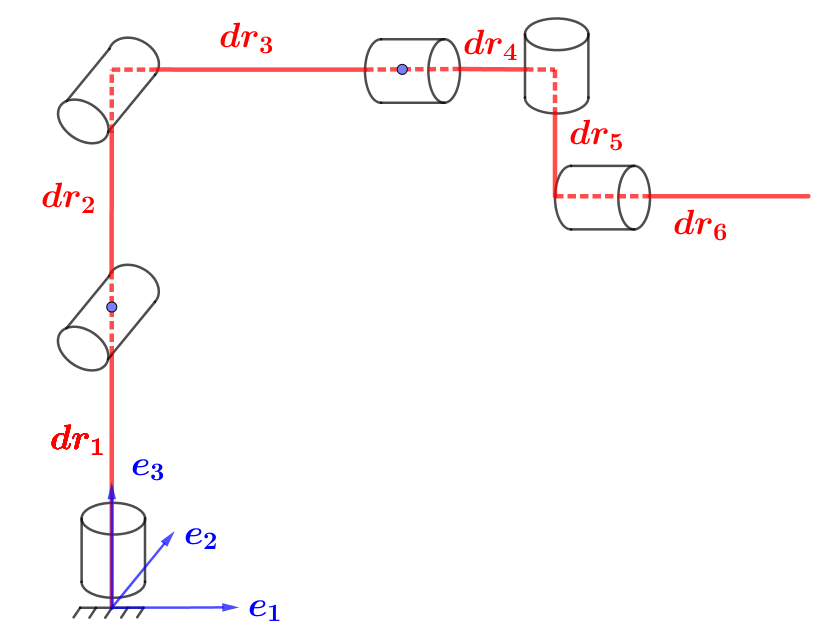
\includegraphics[scale=0.32]{6RGeo.png}
        \caption{Schéma du robot 6R en configuration initiale}
    \end{minipage}
\end{figure}


Il y a donc six bras, avec 6 rotations d'axe (dans l'ordre) $\et$, $\ed$, $\ed$, $\eu$, $\et$ et $\eu$. 

En notant $dr_i$ la longueur du bras $i$, pour $i\in \lbrace 1,2,3, 4, 5, 6 \rbrace$, on obtient en Coq les définitions suivantes : 

\begin{figure}[!ht]
\centering
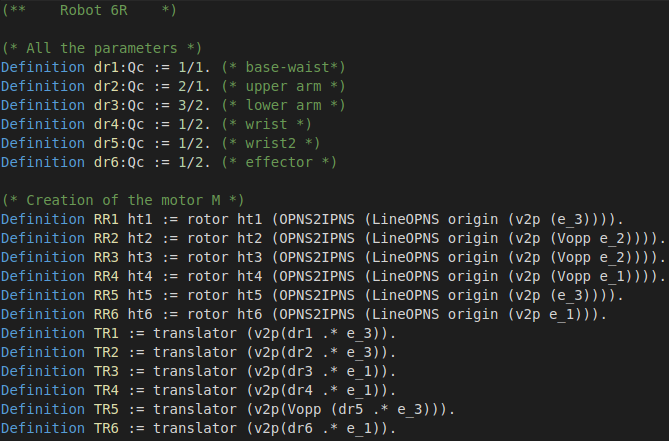
\includegraphics[scale=0.5]{6RParam.png}
\caption{Paramètres du robot 6R}
\end{figure}
\newpage
Le robot 6R est créé et testé comme précédemment, avec des angles de $\theta_1 \approx 106.26 ^{\circ}$, $\theta_2 \approx 134.76 ^{\circ}$, $\theta_3 \approx 123.86^\circ$, $\theta_4 \approx 147.48^\circ$, $\theta_5 \approx 92.79^\circ$, $\theta_6 \approx 142.15^\circ$ (toujours parce que les demi-angles ont un cosinus et un sinus rationnels). L'angle $\theta_6$ n'influe pas sur la position finale de l'effecteur, mais à nouveau sur sa direction. 
\begin{figure}[!ht]
\centering
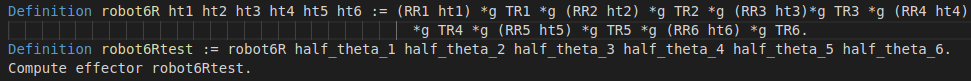
\includegraphics[scale=0.5]{6RDef.png}
\caption{Définition et test du robot 6R}
\end{figure}

On trouve : 
\begin{figure}[!ht]
\centering
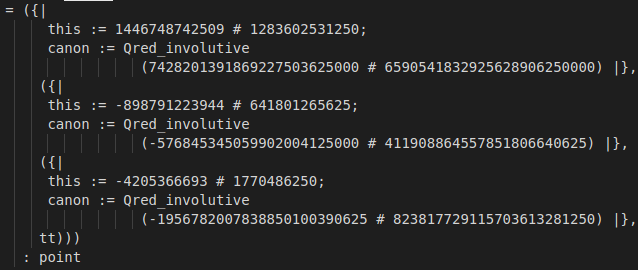
\includegraphics[scale=0.35]{6RRes.png}
\caption{Résultat du test du robot 6R}
\end{figure}

La position de l'effecteur est donc approximativement de $(1.13, -1.40, -2.38)$.

Testons encore sur CLUCalc. Voici le robot avec la position testée : 

\begin{figure}[!ht]
\centering
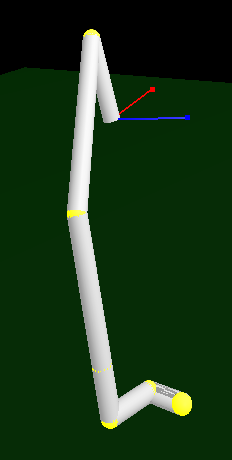
\includegraphics[scale=0.75]{6RCluCalc.png}
\caption{robot 6R construit en CLUCalc}
\end{figure}

Et la position finale de l'effecteur (et des points de liaison intermédiaires) :

\begin{figure}[!ht]
\centering
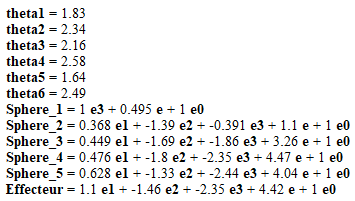
\includegraphics[scale=0.65]{6RCluRes.png}
\caption{Position de l'effecteur du 6R en CLUCalc}
\end{figure}

On voit que la position est toujours correcte, aux arrondis près. 

\subsubsection{Conclusion }

On a donc dans cette partie créé en Coq les robots considérés et vérifié que pour ces trois robots, le résultat renvoyé par Coq est bien celui renvoyé par CLUCalc. Tout ceci a uniquement été fait en utilisant les algèbres géométriques conformes. Cela aurait bien sûr aussi pu être fait à partir de la géométrie classique, mais on peut observer ici la simplicité des opérations utilisées. 

\subsection{Cinématique inverse}

Dans cette partie-là, nous allons nous intéresser au problème inverse. Nous allons nous donner une position finale à atteindre, et trouver quels sont les angles et les longueurs des translations à mettre à nos différents paramètres pour atteindre ce point. Lors de ce problème, plusieurs difficultés peuvent apparaître : 
\begin{itemize}
\item Le point considéré est inatteignable. Pour considérer un point atteignable, on peut se référer à la documentation du robot qui devrait donner le rayon d'action de ce robot, ou calculer celui-ci nous-mêmes. 
Dans le cas du robot SCARA par exemple, on peut voir que l'ensemble des points atteignables est l'ensemble des points de coordonnées $$(x,y,z)\text{ avec } |l_2-l_1|^2 \leq x^2+y^2 \leq (l_1+l_2)^2 \text{ et } z\in [-l_{3,max}-l_4, -l_4] $$ $\text{où } l_{3,max}$ est la longueur maximale du vérin effectuant la translation. En effet, pour la cote, c'est évident, et pour les deux premières coordonnées, on peut se référer au dessin ci-dessous, représentant le robot SCARA vu de dessus : 
\newpage

\begin{figure}[!ht]
\centering
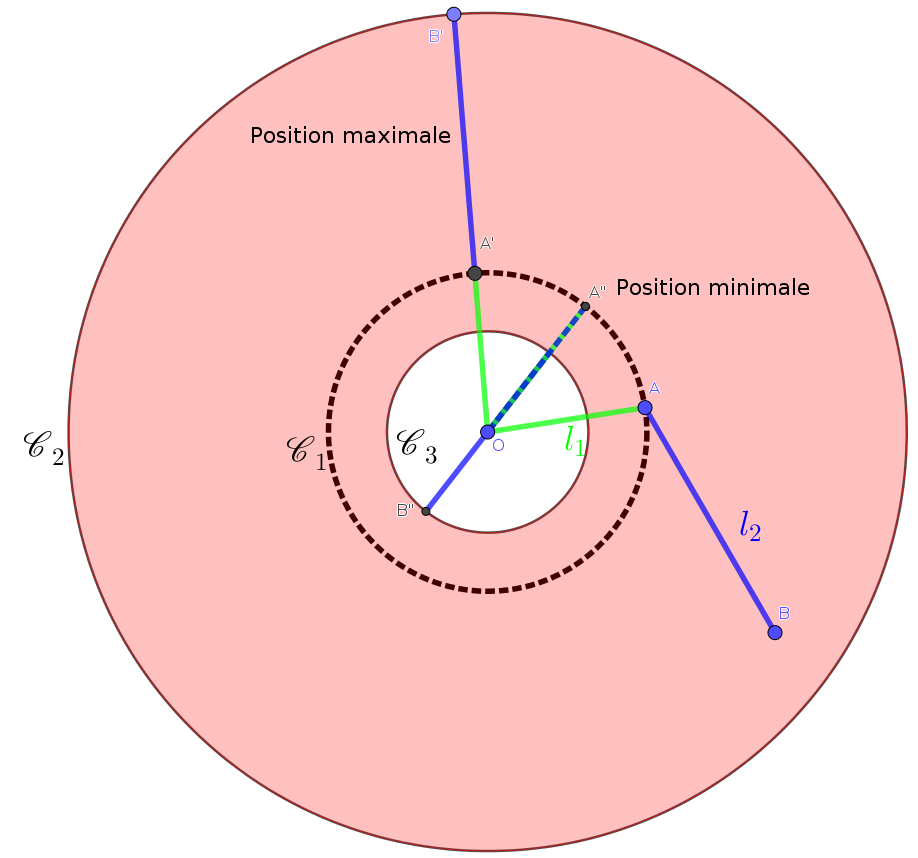
\includegraphics[scale=0.35]{SCARADessus.png}
\caption{Robot SCARA vu de dessus.}
\end{figure}

Les bras $[OA]$ et $[AB]$ sont en position quelconque. Le point $A$ peut décrire le cercle $\mathscr{C}_1$. Au maximum (cas représenté sur la figure par les points $O$, $A'$ et $B'$), le deuxième bras est parallèle au premier et de même sens. Le point $B$ décrit dans ce cas le cercle $\mathscr{C}_2$ . 

Au minimum (cas représenté sur la figure par les points $O$, $A''$ et $B''$), le deuxième bras est parallèle au premier et de sens contraire. Le point $B$ décrit dans ce cas le cercle $\mathscr{C}_3$ . 

L'anneau rouge correspond donc à l'ensemble des points atteignables par le robot SCARA. 

\item Il peut y avoir plusieurs solutions, même une infinité. Par exemple, pour le robot SCARA, si un point est atteignable et strictement compris dans l'anneau rouge au-dessus, il y aura toujours deux façons d'atteindre le point considéré. Le point $A$ se situe à l'une des deux intersections du cercle de centre $O$ et de rayon $l_1$, et de celui de centre $B$ et de rayon $l_2$ : \newpage

\begin{figure}[!ht]
\centering
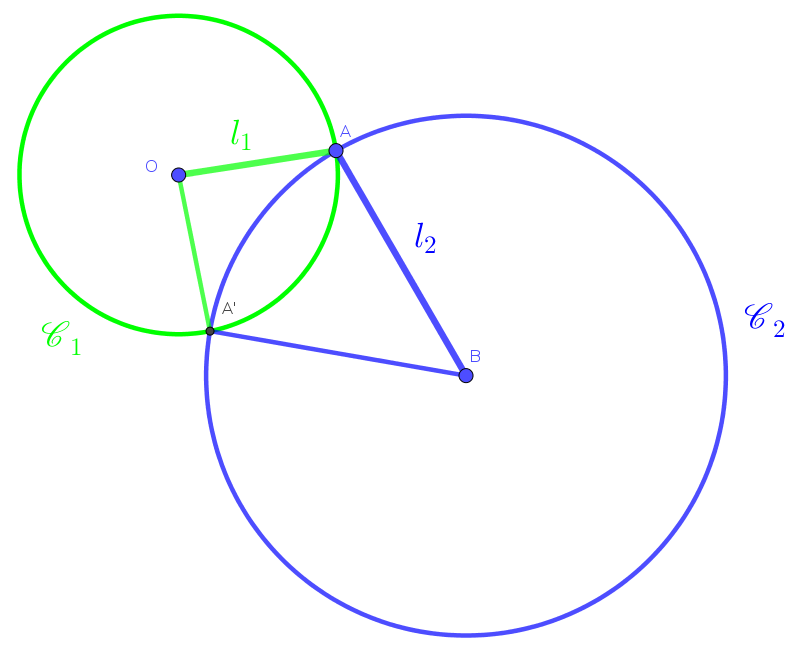
\includegraphics[scale=0.35]{SCARADessus2.png}
\caption{Les deux points $A$ et $A'$ permettent d'atteindre le point $B$.}
\label{SCARA}
\end{figure}

Pour le robot 6R, ayant 6 degrés de liberté, il y a une infinité de façons d'atteindre un point atteignable donné. Mais ici, également la direction finale de l'effecteur va nous intéresser, ainsi le problème de la cinématique inverse pour ce robot sera en fait de trouver les angles à donner aux différents bras pour avoir l'effecteur à la position et dans la direction voulue. Ce problème aura aussi plusieurs solutions, à cause de phénomènes similaires à celui du robot SCARA.
\end{itemize}

\subsubsection{Robot SCARA}

Nous avons déjà vu que l'ensemble des points atteignables est donné par 
$$E = \left \lbrace (x,y,z)\in \R^3 : |l_2-l_1|^2 \leq x^2+y^2 \leq (l_1+l_2)^2 \text{ et } z\in [-l_{3,max}-l_4, l_4]\right \rbrace$$

Soit donc $(x,y,z)\in E$. On cherche donc deux angles $\theta_1$ et $\theta_2$ dans $]-\pi, \pi]$ et une longueur $l_3 \in [0,l_{3,max}]$ tels que l'effecteur soit en position $(x,y,z)$. 

\begin{figure}[!ht]
\centering
\includegraphics[scale=0.35]{SCARAIK.png}
\end{figure}

On voit de façon évidente que les angles ne vont pas influer sur la côte, et donc comme $z=-l_3-l_4$, on peut déjà en déduire que $l_3 = -z-l_4$. 

Il reste à trouver les deux angles. Pour cela, on va d'abord trouver les coordonnées du point $A$ : 

\begin{itemize}
\item On sait que ce point est sur le plan $P$ d'équation $z=0$. 
\item Sa distance à $O$ est de $l_1$, donc il est situé sur la sphère $S_1$ de centre $O$ de rayon $l_1$. 
\item Le point $B$ a pour coordonnées $(x,y,0)$, et $A$ est situé à une distance de $l_2$ de $B$, donc $A$ est sur la sphère $S_2$ de centre $B$ de rayon $l_2$. 
\end{itemize}

\begin{figure}[!ht]
\centering
\includegraphics[scale=0.45]{SCARAIK2.png}
\caption{L'intersection des deux sphères (le cercle jaune) et du plan $z=0$ (en vert clair) donne deux points : un dessiné en bleu, le bras est sur l'autre.}
\end{figure}

Au final, pour avoir l'emplacement du point $A$, il suffit avec les algèbres géométriques de calculer $$P \wedge S_1 \wedge S_2$$
où $P=\et$, $S_1 = - \frac{1}{2}l_1^2\ei+\ez$ et $S_2 = x\eu+y\ed +\frac{1}{2}(x^2+ y^2-l_2^2)\ei+\ez$ d'après les formules du tableau \ref{tableau}.

Ceci renverra une paire de points (notée $Pp$) car il y a deux solutions, comme vu au-dessus. Pour en choisir un, il faut calculer $\frac{Pp^* \pm \sqrt{Pp^* \cdot Pp^*} }{\ei \cdot Pp^*}$ (voir \cite{Dietmar} pour plus de détails), le signe choisi donnant un point ou l'autre. 

Voici les calculs effectué en CLUCalc ainsi que les résultats obtenus : \newpage

\begin{figure}[!ht]
    \begin{minipage}[c]{.46\linewidth}
        \centering
        \includegraphics[scale=0.81]{SCARAIK3.png}
        \caption{Les calculs}
    \end{minipage}
    \hfill%
    \begin{minipage}[c]{.46\linewidth}
        \centering
        \includegraphics[scale=0.8]{SCARAIK4.png}
        \caption{Les résultats}
    \end{minipage}
\end{figure}

On remarque qu'effectivement un des deux points de la paire de points a les mêmes coordonnées que le point $A$. 

Sur le dessin de la figure \ref{SCARA}, la longueur $AB$ mesure $\sqrt{x^2+y^2}$, et on a $\theta_1 = (\overrightarrow{OA}, \overrightarrow{OB})$ et $\theta_2 = (\overrightarrow{AO}, \overrightarrow{AB})$.

Pour obtenir les angles correspondants, il reste à utiliser les formules d'Al-Kashi :  $$\theta_1 = arccos \left(\frac{l_1^2+AB^2-l_2^2}{2 l_1 AB}\right)\text{ et }\theta_2 = arccos \left(\frac{l_1^2+l_2^2-AB^2}{2 l_1 l_2}\right)$$





\section{Conclusion}

\subsection{Synthèse}

Nous avons donc vu dans ce mémoire comment les algèbres géométriques ont permis par des raisonnements relativement simples (une fois le concept compris) de calculer l'emplacement de différents bras de robots à partir des paramètres (cinématique directe) et comment à partir de l'emplacement final déterminer les paramètres de départ (cinématique indirecte).

Le logiciel assistant de preuve Coq a permis de démontrer certains résultats sur ces algèbres géométriques et de faire le lien entre cette géométrie et la géométrie "classique". Ce logiciel a également permis de "créer" virtuellement ces robots pour calculer la cinématique directe ou indirecte à partir des donnés initiales. 

Tout ce qui a été expliqué dans ce mémoire a été soit démontré en Coq, soit vérifié empiriquement sur le logiciel CLUCalc. 

\subsection{Difficultés rencontrées - Perspectives }

Comme vu plus haut, la manipulation des réels en Coq est extrêmement compliquée, surtout lorsqu'il s'agit de faire des calculs avec. Dans le cas de la cinématique inverse, pour choisir un point à partir d'une paire de points, il nous faut une formule contenant une racine carrée. Il n'est donc plus suffisant dans ce cas de travailler sur les rationnels, car la partie sous la racine ne sera pas dans le cas général un carré de rationnel.

Nous avons implémenté le même code adapté pour les réels en Coq, mais ceci ne permet pas de faire les calculs avec, juste de retrouver les résultats théoriques. En effet, la bibliothèque des réels en coq n'est pas prévue pour faire des calculs (par exemple les nombres 0 et 1 sont définis, mais pas 2 !). 

Nous avons également essayé avec les bibliothèques Interval et C-CoRN de Coq de faire calculer des intervalles qui contiendraient la bonne valeur, mais cela n'a pas été concluant non plus. 

Une fois ce problème surmonté, il serait intéressant de démontrer qu'appliquer la cinématique indirecte puis la cinématique directe aboutit bien à la situation de départ. 

Une autre perspective serait de trouver un chemin pour l'effecteur d'un point à un autre sans passer par une région qui serait interdite (même toutes les parties du robot, pas seulement l'effecteur, ne pourraient pas passer par cette région). 




\nocite{*}
\bibliographystyle{unsrt}
\bibliography{biblio}
\end{document}